\documentclass[]{elsarticle} %review=doublespace preprint=single 5p=2 column
%%% Begin My package additions %%%%%%%%%%%%%%%%%%%
\usepackage[hyphens]{url}
\usepackage{lineno} % add
\providecommand{\tightlist}{%
  \setlength{\itemsep}{0pt}\setlength{\parskip}{0pt}}

\bibliographystyle{elsarticle-harv}
\biboptions{sort&compress} % For natbib
\usepackage{graphicx}
\usepackage{booktabs} % book-quality tables
%% Redefines the elsarticle footer
%\makeatletter
%\def\ps@pprintTitle{%
% \let\@oddhead\@empty
% \let\@evenhead\@empty
% \def\@oddfoot{\it \hfill\today}%
% \let\@evenfoot\@oddfoot}
%\makeatother

% A modified page layout
\textwidth 6.75in
\oddsidemargin -0.15in
\evensidemargin -0.15in
\textheight 9in
\topmargin -0.5in
%%%%%%%%%%%%%%%% end my additions to header

\usepackage[T1]{fontenc}
\usepackage{lmodern}
\usepackage{amssymb,amsmath}
\usepackage{ifxetex,ifluatex}
\usepackage{fixltx2e} % provides \textsubscript
% use upquote if available, for straight quotes in verbatim environments
\IfFileExists{upquote.sty}{\usepackage{upquote}}{}
\ifnum 0\ifxetex 1\fi\ifluatex 1\fi=0 % if pdftex
  \usepackage[utf8]{inputenc}
\else % if luatex or xelatex
  \usepackage{fontspec}
  \ifxetex
    \usepackage{xltxtra,xunicode}
  \fi
  \defaultfontfeatures{Mapping=tex-text,Scale=MatchLowercase}
  \newcommand{\euro}{€}
\fi
% use microtype if available
\IfFileExists{microtype.sty}{\usepackage{microtype}}{}
\usepackage{longtable}
\usepackage{graphicx}
% We will generate all images so they have a width \maxwidth. This means
% that they will get their normal width if they fit onto the page, but
% are scaled down if they would overflow the margins.
\makeatletter
\def\maxwidth{\ifdim\Gin@nat@width>\linewidth\linewidth
\else\Gin@nat@width\fi}
\makeatother
\let\Oldincludegraphics\includegraphics
\renewcommand{\includegraphics}[1]{\Oldincludegraphics[width=\maxwidth]{#1}}
\ifxetex
  \usepackage[setpagesize=false, % page size defined by xetex
              unicode=false, % unicode breaks when used with xetex
              xetex]{hyperref}
\else
  \usepackage[unicode=true]{hyperref}
\fi
\hypersetup{breaklinks=true,
            bookmarks=true,
            pdfauthor={},
            pdftitle={A dynamic bioenergetic model for coral-Symbiodinium symbioses and coral bleaching as an alternate stable state},
            colorlinks=true,
            urlcolor=blue,
            linkcolor=magenta,
            pdfborder={0 0 0}}
\urlstyle{same}  % don't use monospace font for urls
\setlength{\parindent}{0pt}
\setlength{\parskip}{6pt plus 2pt minus 1pt}
\setlength{\emergencystretch}{3em}  % prevent overfull lines
\setcounter{secnumdepth}{0}
% Pandoc toggle for numbering sections (defaults to be off)
\setcounter{secnumdepth}{0}
% Pandoc header


\usepackage[nomarkers]{endfloat}

\begin{document}
\begin{frontmatter}

  \title{A dynamic bioenergetic model for coral-\emph{Symbiodinium} symbioses and
coral bleaching as an alternate stable state}
    \author[HIMB]{Ross Cunning\corref{c1}}
   \ead{ross.cunning@gmail.com} 
   \cortext[c1]{Corresponding Author}
    \author[UCSB,MSI]{Erik B. Muller}
  
  
    \author[HIMB]{Ruth D. Gates}
  
  
    \author[UCSB]{Roger M. Nisbet}
  
  
      \address[HIMB]{Hawaii Institute of Marine Biology, School of Ocean and Earth Science
and Technology, University of Hawaii at Manoa, USA}
    \address[UCSB]{Department of Ecology, Evolution, and Marine Biology, University of
California, Santa Barbara, USA}
    \address[MSI]{Marine Science Institute, University of California, Santa Barbara, USA}
  
  \begin{abstract}
  Coral reef ecosystems owe their ecological success--and vulnerability to
  climate change--to the symbiotic metabolism of corals and
  \emph{Symbiodinium} spp. The urgency to understand and predict the
  stability and breakdown of these symbioses (i.e., coral `bleaching')
  demands the development and application of theoretical tools. Here, we
  develop a dynamic bioenergetic model of coral-\emph{Symbiodinium}
  symbioses that demonstrates realistic steady-state patterns in coral
  growth and symbiont abundance across gradients of light, nutrients, and
  feeding. Furthermore, by including a mechanistic treatment of
  photo-oxidative stress, the model displays dynamics of bleaching and
  recovery that can be explained as transitions between alternate stable
  states. These dynamics reveal that `healthy' and `bleached' states
  correspond broadly to nitrogen- and carbon-limitation in the system,
  with transitions between them occurring as integrated responses to
  multiple environmental factors. Indeed, a suite of complex emergent
  behaviors reproduced by the model (e.g., bleaching is exacerbated by
  nutrients and attenuated by feeding) suggests it captures many important
  attributes of the system; meanwhile, its modular framework and open
  source R code are designed to facilitate further problem-specific
  development. We see significant potential for this modeling framework to
  generate testable hypotheses and predict integrated, mechanistic
  responses of corals to environmental change, with important implications
  for understanding the performance and maintenance of symbiotic systems.
  \end{abstract}
  
 \end{frontmatter}

\section{Introduction}\label{introduction}

The nutritional exchange between corals and \emph{Symbiodinium} directly
underlies the capacity of corals to build coral reef ecosystems, worth
trillions of US Dollars annually (Costanza, Groot, and Sutton 2014).
However, the complex symbiotic metabolism of corals is vulnerable to
disruption by numerous anthropogenic environmental perturbations,
jeopardizing their future persistence. In order to understand and
predict responses of corals to complex changes in their environment, a
mechanistic understanding of how multiple interacting factors drive the
individual and emergent physiology of both symbiotic partners is
necessary. Such a task is well suited for theoretical modeling
frameworks such as Dynamic Energy Budget (DEB) theory (Kooijman 2010),
although the complexity of such theory makes these efforts inaccessible
to many biologists (Jager, Martin, and Zimmer 2013). In order to bridge
this gap, we present here a simplified dynamic bioenergetic model for
coral-\emph{Symbiodinium} symbioses that aims to mechanistically
integrate the impacts of complex environmental change on the
physiological performance of reef corals, including responses to
environmental stress.

In reef coral symbioses, intracellular \emph{Symbiodinium} translocate
photosynthetically fixed carbon to support coral metabolism, while the
animal host provides access to inorganic nutrients and carbon dioxide
(Muscatine and Porter 1977). Previous application of DEB theory to this
syntrophic system (Muller et al. 2009) demonstrated a stable symbiotic
relationship and qualitatively realistic growth and biomass ratios
across gradients of ambient irradiance, nutrients, and food. This model
(as well as the present work) assumes that 1) \emph{Symbiodinium} has
priority access to fixed carbon through photosynthesis, 2) the coral
animal has priority access to nitrogen through contact with seawater and
feeding on prey, and 3) each partner shares with the other only what it
cannot use for its own growth. In its simplest form, this principle of
sharing the surplus is sufficient to describe the dynamics of diverse
syntrophic organs and organisms (e.g., trees, duckweeds, corals),
suggesting the mechanism is mathematically and evolutionarily robust
(Nisbet et al., in prep.).

While the formal DEB model of Muller et al. (2009) represents the most
significant theoretical contribution in coral symbiosis research to
date, we aim to strengthen the role of theory and broaden its potential
application in three primary ways:

\begin{enumerate}
\def\labelenumi{\arabic{enumi}.}
\item
  \emph{Develop a new module of photo-oxidative stress.} Of primary
  interest to coral biologists and ecologists is symbiosis dysfunction
  under environmental stress, resulting in coral ``bleaching''--the loss
  of algal symbionts from the association (Jokiel and Coles 1977).
  Bleaching is thought to be triggered by photo-oxidative stress in
  \emph{Symbiodinium} (Weis 2008), which has been modeled previously as
  a response to absolute external irradiance (Eynaud, Nisbet, and Muller
  2011). However, this response may also depend on self-shading by other
  symbionts (Enríquez, Méndez, and Iglesias-Prieto 2005),
  CO\textsubscript{2} availability at the site of photosynthesis
  (Wooldridge 2009), and other non-photochemical quenching mechanisms
  (Roth 2014). We incorporate these features into a new photo-oxidative
  stress module linking overreduction of the photosynthetic light
  reactions to downstream impacts of photoinhibition and photodamage.
  Importantly, this formulation introduces a link between
  CO\textsubscript{2}-limitation of photosynthesis and bleaching, and
  potential synergistic roles for heterotrophy and nutrient availability
  in influencing bleaching responses (Wooldridge 2014b)
\item
  \emph{Reduce theoretical and mathematical complexity.} Following the
  logic of Jager, Martin, and Zimmer (2013), we exclude certain features
  of formal DEB theory in order to capture behaviors of interest with
  the simplest possible formulation. Here, we present a model without
  reserves, maturity, or reproduction (see Kooijman 2010). This
  formulation precludes modeling the full life cycle of corals as
  reproduction, larval stages, and metamorphosis are not considered, but
  greatly reduces theoretical complexity and parameter numbers, which is
  advantageous given the relative paucity of data for corals. Moreover,
  dynamics of the symbiosis (i.e., changes in symbiont to host biomass,
  including bleaching and recovery) and coral biomass growth are
  efficiently captured with this simpler formulation, which also
  increases accessibility for biologists and ecologists without
  requiring expertise in DEB theory.
\item
  \emph{Provide well-documented, open source code.} In order to
  facilitate the continued development and application of theoretical
  modeling tools for coral symbioses, we provide access to the model in
  the form of an R package called coRal
  \url{github.com/jrcunning/coRal}, which users may install to run and
  visualize model simulations. With an accessible and modular framework,
  we envision this code base as a resource for further development by
  the scientific community to include additional complexity and
  problem-specific components. We chose R (R Core Team 2014), an open
  source programming language in common use by biologists and
  ecologists, to reach the widest possible audience with this work.
\end{enumerate}

With these as our primary motivations, we describe a simplified approach
to bioenergetic modeling of coral-\emph{Symbiodinium} symbioses that
dynamically integrates the influences of external irradiance, nutrients,
and prey availability on coral growth and symbiosis dynamics (i.e.,
changes in symbiont:host biomass ratios), allowing for the possibility
of coral bleaching in response to photooxidative stress. An emergent
finding of this work is that coral bleaching can be interpreted as an
alternate stable state of the symbiotic system, which provides a new
framework for understanding the mechanisms that drive a coral into a
bleached state, as well as those that facilitate recovery. In the
following sections, we describe and provide rationale for the model
structure, demonstrate a range of steady state and dynamic behaviors
that are consistent with observed phenomena, and discuss new insights
from this work in understanding responses of coral-\emph{Symbiodinium}
symbioses to environmental change.

\section{Model description}\label{model-description}

In this dynamical system, both the coral host and algal symbiont acquire
and use carbon and nitrogen to construct biomass. The symbiont fixes
carbon through photosynthesis and receives nitrogen shared by the host,
while the host acquires nitrogen from the environment and receives
carbon shared by the symbiont. A graphical representation of the model
is presented in Fig. 1, and each model flux and parameter is defined in
Tables 1 and 2, respectively. We use C-moles (C-mol) as the unit of
biomass for consistency with the rigorous mass balance of DEB theory: 1
C-mol is equivalent to the amount of biomass containing 1 mole of carbon
atoms. Host biomass (expressed as C-mol H), symbiont biomass (expressed
as C-mol S), and prey biomass (expressed as C-mol X) have fixed, but
different, molar N:C ratios (Table 2), consistent with the assumption of
strong homeostasis in DEB theory (Kooijman 2010). Biomass is produced
from carbon and nitrogen by parallel complementary synthesizing units
(SUs) -- mathematical specifications of the formation of a product by a
metabolic network processing two complementary substrates in parallel
(Kooijman (2010), p.~105, Fig. 3.7). The two state variables in the
model are symbiont biomass and coral biomass; because resources are
acquired proportionally to surface area, and surface area is
proportional to volume (corals are V1-morphs in a DEB context (Kooijman
(2010), p.~122)), biomass increases exponentially during growth (indeed,
corals grow exponentially (Bak 1976)).

Environmental stress is implemented in the form of photooxidative
stress, which is thought to be a primary trigger of coral bleaching
(Lesser 1997; Weis 2008; Wooldridge 2009). To simulate bleaching, we
model the absorption and quenching of light energy by photochemistry and
non-photochemical quenching, and the responses that occur (i.e.,
photoinhibition, photodamage, and symbiont loss) when these quenching
capacities are overwhelmed. While bleaching in response to high light
alone has been observed experimentally (Schutter et al. 2011; Downs et
al. 2013), mass coral bleaching events occur concurrently with high
temperature (Hoegh-Guldberg 1999). Thus, it is important to justify our
consideration of light as the primary stressor. In reality, light and
temperature interact synergistically (Coles and Jokiel 1978; Jones et
al. 1998), and in fact, any stressor that disrupts the quenching of
light energy may lead to bleaching (Wooldridge 2010; Baker and Cunning
2015). This is because the proximate cause of photo-oxidative stress is
excess excitation energy, but the upstream events that lead to this
situation may be diverse. Indeed, elevated temperature may inhibit
Rubisco functioning (Jones et al. 1998) and the repair of the D1 protein
in photosystem II (Warner, Fitt, and Schmidt 1999), which reduces the
capacity of photochemical quenching and leads to an excess of light
energy. In this way, elevated temperature serves to reduce the threshold
above which light stresses the system (Hoegh-Guldberg 1999);
importantly, light is still the proximate stressor. Therefore, we
omitted temperature from the model to maintain a desired level of
simplicity, while still allowing photooxidative stress and bleaching to
be simulated with biological realism in response to light.

Table 1. Model fluxes (mass-specific). Units are explained in the text.
(Abbreviations: CCMs=carbon concentrating mechanisms;
NPQ=non-photochemical quenching; ROS=reactive oxygen species)

\begin{longtable}[c]{@{}llll@{}}
\toprule
\begin{minipage}[b]{0.10\columnwidth}\raggedright\strut
Symbol
\strut\end{minipage} &
\begin{minipage}[b]{0.45\columnwidth}\raggedright\strut
Description
\strut\end{minipage} &
\begin{minipage}[b]{0.27\columnwidth}\raggedright\strut
Units
\strut\end{minipage} &
\begin{minipage}[b]{0.10\columnwidth}\raggedright\strut
Eq. no.
\strut\end{minipage}\tabularnewline
\midrule
\endhead
\begin{minipage}[t]{0.10\columnwidth}\raggedright\strut
\(j_X\)
\strut\end{minipage} &
\begin{minipage}[t]{0.45\columnwidth}\raggedright\strut
Prey assimilation (feeding) rate
\strut\end{minipage} &
\begin{minipage}[t]{0.27\columnwidth}\raggedright\strut
C-mol X C-mol H\textsuperscript{-1} d\textsuperscript{-1}
\strut\end{minipage} &
\begin{minipage}[t]{0.10\columnwidth}\raggedright\strut
3
\strut\end{minipage}\tabularnewline
\begin{minipage}[t]{0.10\columnwidth}\raggedright\strut
\(j_N\)
\strut\end{minipage} &
\begin{minipage}[t]{0.45\columnwidth}\raggedright\strut
Nitrogen uptake rate
\strut\end{minipage} &
\begin{minipage}[t]{0.27\columnwidth}\raggedright\strut
mol N Cmol H\textsuperscript{-1} d\textsuperscript{-1}
\strut\end{minipage} &
\begin{minipage}[t]{0.10\columnwidth}\raggedright\strut
4
\strut\end{minipage}\tabularnewline
\begin{minipage}[t]{0.10\columnwidth}\raggedright\strut
\(j_{HG}\)
\strut\end{minipage} &
\begin{minipage}[t]{0.45\columnwidth}\raggedright\strut
Host biomass formation rate
\strut\end{minipage} &
\begin{minipage}[t]{0.27\columnwidth}\raggedright\strut
C-mol H C-mol H\textsuperscript{-1} d\textsuperscript{-1}
\strut\end{minipage} &
\begin{minipage}[t]{0.10\columnwidth}\raggedright\strut
5
\strut\end{minipage}\tabularnewline
\begin{minipage}[t]{0.10\columnwidth}\raggedright\strut
\(j_{HT}\)
\strut\end{minipage} &
\begin{minipage}[t]{0.45\columnwidth}\raggedright\strut
Host biomass turnover rate
\strut\end{minipage} &
\begin{minipage}[t]{0.27\columnwidth}\raggedright\strut
C-mol H C-mol H\textsuperscript{-1} d\textsuperscript{-1}
\strut\end{minipage} &
\begin{minipage}[t]{0.10\columnwidth}\raggedright\strut
6
\strut\end{minipage}\tabularnewline
\begin{minipage}[t]{0.10\columnwidth}\raggedright\strut
\(r_{NH}\)
\strut\end{minipage} &
\begin{minipage}[t]{0.45\columnwidth}\raggedright\strut
Recycled nitrogen from host turnover
\strut\end{minipage} &
\begin{minipage}[t]{0.27\columnwidth}\raggedright\strut
mol N C-mol H\textsuperscript{-1} d\textsuperscript{-1}
\strut\end{minipage} &
\begin{minipage}[t]{0.10\columnwidth}\raggedright\strut
7
\strut\end{minipage}\tabularnewline
\begin{minipage}[t]{0.10\columnwidth}\raggedright\strut
\(\rho_N\)
\strut\end{minipage} &
\begin{minipage}[t]{0.45\columnwidth}\raggedright\strut
Nitrogen shared with the symbiont
\strut\end{minipage} &
\begin{minipage}[t]{0.27\columnwidth}\raggedright\strut
mol N C-mol H\textsuperscript{-1} d\textsuperscript{-1}
\strut\end{minipage} &
\begin{minipage}[t]{0.10\columnwidth}\raggedright\strut
8
\strut\end{minipage}\tabularnewline
\begin{minipage}[t]{0.10\columnwidth}\raggedright\strut
\(j_{eC}\)
\strut\end{minipage} &
\begin{minipage}[t]{0.45\columnwidth}\raggedright\strut
Excess carbon used to activate host CCMs
\strut\end{minipage} &
\begin{minipage}[t]{0.27\columnwidth}\raggedright\strut
mol C C-mol H\textsuperscript{-1} d\textsuperscript{-1}
\strut\end{minipage} &
\begin{minipage}[t]{0.10\columnwidth}\raggedright\strut
9
\strut\end{minipage}\tabularnewline
\begin{minipage}[t]{0.10\columnwidth}\raggedright\strut
\(j_{CO_2}\)
\strut\end{minipage} &
\begin{minipage}[t]{0.45\columnwidth}\raggedright\strut
CO\textsubscript{2} input to photosynthesis
\strut\end{minipage} &
\begin{minipage}[t]{0.27\columnwidth}\raggedright\strut
mol CO\textsubscript{2} C-mol H\textsuperscript{-1}
d\textsuperscript{-1}
\strut\end{minipage} &
\begin{minipage}[t]{0.10\columnwidth}\raggedright\strut
10
\strut\end{minipage}\tabularnewline
\begin{minipage}[t]{0.10\columnwidth}\raggedright\strut
\(j_L\)
\strut\end{minipage} &
\begin{minipage}[t]{0.45\columnwidth}\raggedright\strut
Light absorption rate
\strut\end{minipage} &
\begin{minipage}[t]{0.27\columnwidth}\raggedright\strut
mol photons C-mol S\textsuperscript{-1} d\textsuperscript{-1}
\strut\end{minipage} &
\begin{minipage}[t]{0.10\columnwidth}\raggedright\strut
12
\strut\end{minipage}\tabularnewline
\begin{minipage}[t]{0.10\columnwidth}\raggedright\strut
\(r_{CH}\)
\strut\end{minipage} &
\begin{minipage}[t]{0.45\columnwidth}\raggedright\strut
Recycled CO\textsubscript{2} from host
\strut\end{minipage} &
\begin{minipage}[t]{0.27\columnwidth}\raggedright\strut
mol CO\textsubscript{2} C-mol H\textsuperscript{-1}
d\textsuperscript{-1}
\strut\end{minipage} &
\begin{minipage}[t]{0.10\columnwidth}\raggedright\strut
13
\strut\end{minipage}\tabularnewline
\begin{minipage}[t]{0.10\columnwidth}\raggedright\strut
\(r_{CS}\)
\strut\end{minipage} &
\begin{minipage}[t]{0.45\columnwidth}\raggedright\strut
Recycled CO\textsubscript{2} from symbiont
\strut\end{minipage} &
\begin{minipage}[t]{0.27\columnwidth}\raggedright\strut
mol CO\textsubscript{2} C-mol S\textsuperscript{-1}
d\textsuperscript{-1}
\strut\end{minipage} &
\begin{minipage}[t]{0.10\columnwidth}\raggedright\strut
14
\strut\end{minipage}\tabularnewline
\begin{minipage}[t]{0.10\columnwidth}\raggedright\strut
\(j_{CP}\)
\strut\end{minipage} &
\begin{minipage}[t]{0.45\columnwidth}\raggedright\strut
Photosynthesis rate
\strut\end{minipage} &
\begin{minipage}[t]{0.27\columnwidth}\raggedright\strut
mol C C-mol S\textsuperscript{-1} d\textsuperscript{-1}
\strut\end{minipage} &
\begin{minipage}[t]{0.10\columnwidth}\raggedright\strut
15
\strut\end{minipage}\tabularnewline
\begin{minipage}[t]{0.10\columnwidth}\raggedright\strut
\(j_{eL}\)
\strut\end{minipage} &
\begin{minipage}[t]{0.45\columnwidth}\raggedright\strut
Light energy in excess of photochemistry
\strut\end{minipage} &
\begin{minipage}[t]{0.27\columnwidth}\raggedright\strut
mol photons C-mol S\textsuperscript{-1} d\textsuperscript{-1}
\strut\end{minipage} &
\begin{minipage}[t]{0.10\columnwidth}\raggedright\strut
16
\strut\end{minipage}\tabularnewline
\begin{minipage}[t]{0.10\columnwidth}\raggedright\strut
\(j_{NPQ}\)
\strut\end{minipage} &
\begin{minipage}[t]{0.45\columnwidth}\raggedright\strut
Total capacity of NPQ
\strut\end{minipage} &
\begin{minipage}[t]{0.27\columnwidth}\raggedright\strut
mol photons C-mol S\textsuperscript{-1} d\textsuperscript{-1}
\strut\end{minipage} &
\begin{minipage}[t]{0.10\columnwidth}\raggedright\strut
17
\strut\end{minipage}\tabularnewline
\begin{minipage}[t]{0.10\columnwidth}\raggedright\strut
\(c_{ROS}\)
\strut\end{minipage} &
\begin{minipage}[t]{0.45\columnwidth}\raggedright\strut
ROS production proportional to baseline
\strut\end{minipage} &
\begin{minipage}[t]{0.27\columnwidth}\raggedright\strut
--
\strut\end{minipage} &
\begin{minipage}[t]{0.10\columnwidth}\raggedright\strut
18
\strut\end{minipage}\tabularnewline
\begin{minipage}[t]{0.10\columnwidth}\raggedright\strut
\(r_{NS}\)
\strut\end{minipage} &
\begin{minipage}[t]{0.45\columnwidth}\raggedright\strut
Recycled nitrogen from symbiont turnover
\strut\end{minipage} &
\begin{minipage}[t]{0.27\columnwidth}\raggedright\strut
mol N C-mol S\textsuperscript{-1} d\textsuperscript{-1}
\strut\end{minipage} &
\begin{minipage}[t]{0.10\columnwidth}\raggedright\strut
19
\strut\end{minipage}\tabularnewline
\begin{minipage}[t]{0.10\columnwidth}\raggedright\strut
\(j_{SG}\)
\strut\end{minipage} &
\begin{minipage}[t]{0.45\columnwidth}\raggedright\strut
Symbiont biomass formation rate
\strut\end{minipage} &
\begin{minipage}[t]{0.27\columnwidth}\raggedright\strut
C-mol S C-mol S\textsuperscript{-1} d\textsuperscript{-1}
\strut\end{minipage} &
\begin{minipage}[t]{0.10\columnwidth}\raggedright\strut
20
\strut\end{minipage}\tabularnewline
\begin{minipage}[t]{0.10\columnwidth}\raggedright\strut
\(\rho_C\)
\strut\end{minipage} &
\begin{minipage}[t]{0.45\columnwidth}\raggedright\strut
Fixed carbon shared with host
\strut\end{minipage} &
\begin{minipage}[t]{0.27\columnwidth}\raggedright\strut
mol C C-mol S\textsuperscript{-1} d\textsuperscript{-1}
\strut\end{minipage} &
\begin{minipage}[t]{0.10\columnwidth}\raggedright\strut
21
\strut\end{minipage}\tabularnewline
\begin{minipage}[t]{0.10\columnwidth}\raggedright\strut
\(j_{ST}\)
\strut\end{minipage} &
\begin{minipage}[t]{0.45\columnwidth}\raggedright\strut
Symbiont biomass turnover rate
\strut\end{minipage} &
\begin{minipage}[t]{0.27\columnwidth}\raggedright\strut
C-mol S C-mol S\textsuperscript{-1} d\textsuperscript{-1}
\strut\end{minipage} &
\begin{minipage}[t]{0.10\columnwidth}\raggedright\strut
22
\strut\end{minipage}\tabularnewline
\bottomrule
\end{longtable}

Table 2. Model parameters (units explained in the text). Justification
and/or derivation of each parameter value along with supporting
references are provided in the Supplementary Information.
(Abbreviations: CCMs=carbon concentrating mechanisms;
NPQ=non-photochemical quenching; ROS=reactive oxygen species;
DIN=dissolved inorganic nitrogen)

\begin{longtable}[c]{@{}llll@{}}
\toprule
\begin{minipage}[b]{0.10\columnwidth}\raggedright\strut
Symbol
\strut\end{minipage} &
\begin{minipage}[b]{0.45\columnwidth}\raggedright\strut
Description
\strut\end{minipage} &
\begin{minipage}[b]{0.25\columnwidth}\raggedright\strut
Units
\strut\end{minipage} &
\begin{minipage}[b]{0.12\columnwidth}\raggedright\strut
Value
\strut\end{minipage}\tabularnewline
\midrule
\endhead
\begin{minipage}[t]{0.10\columnwidth}\raggedright\strut
\(n_{NH}\)
\strut\end{minipage} &
\begin{minipage}[t]{0.45\columnwidth}\raggedright\strut
N:C molar ratio in host biomass
\strut\end{minipage} &
\begin{minipage}[t]{0.25\columnwidth}\raggedright\strut
--
\strut\end{minipage} &
\begin{minipage}[t]{0.12\columnwidth}\raggedright\strut
\(0.18\)
\strut\end{minipage}\tabularnewline
\begin{minipage}[t]{0.10\columnwidth}\raggedright\strut
\(n_{NS}\)
\strut\end{minipage} &
\begin{minipage}[t]{0.45\columnwidth}\raggedright\strut
N:C molar ratio in symbiont biomass
\strut\end{minipage} &
\begin{minipage}[t]{0.25\columnwidth}\raggedright\strut
--
\strut\end{minipage} &
\begin{minipage}[t]{0.12\columnwidth}\raggedright\strut
\(0.13\)
\strut\end{minipage}\tabularnewline
\begin{minipage}[t]{0.10\columnwidth}\raggedright\strut
\(n_{NX}\)
\strut\end{minipage} &
\begin{minipage}[t]{0.45\columnwidth}\raggedright\strut
N:C molar ratio in prey biomass
\strut\end{minipage} &
\begin{minipage}[t]{0.25\columnwidth}\raggedright\strut
--
\strut\end{minipage} &
\begin{minipage}[t]{0.12\columnwidth}\raggedright\strut
\(0.2\)
\strut\end{minipage}\tabularnewline
\begin{minipage}[t]{0.10\columnwidth}\raggedright\strut
\(j_{HT}^0\)
\strut\end{minipage} &
\begin{minipage}[t]{0.45\columnwidth}\raggedright\strut
Maintenance rate of host biomass
\strut\end{minipage} &
\begin{minipage}[t]{0.25\columnwidth}\raggedright\strut
C-mol H C-mol H\textsuperscript{-1} d\textsuperscript{-1}
\strut\end{minipage} &
\begin{minipage}[t]{0.12\columnwidth}\raggedright\strut
\(0.03\)
\strut\end{minipage}\tabularnewline
\begin{minipage}[t]{0.10\columnwidth}\raggedright\strut
\(j_{ST}^0\)
\strut\end{minipage} &
\begin{minipage}[t]{0.45\columnwidth}\raggedright\strut
Maintenance rate of symbiont biomass
\strut\end{minipage} &
\begin{minipage}[t]{0.25\columnwidth}\raggedright\strut
C-mol S C-mol S\textsuperscript{-1} d\textsuperscript{-1}
\strut\end{minipage} &
\begin{minipage}[t]{0.12\columnwidth}\raggedright\strut
\(0.03\)
\strut\end{minipage}\tabularnewline
\begin{minipage}[t]{0.10\columnwidth}\raggedright\strut
\(\sigma_{NH}\)
\strut\end{minipage} &
\begin{minipage}[t]{0.45\columnwidth}\raggedright\strut
Proportion N turnover recycled in host
\strut\end{minipage} &
\begin{minipage}[t]{0.25\columnwidth}\raggedright\strut
--
\strut\end{minipage} &
\begin{minipage}[t]{0.12\columnwidth}\raggedright\strut
\(0.9\)
\strut\end{minipage}\tabularnewline
\begin{minipage}[t]{0.10\columnwidth}\raggedright\strut
\(\sigma_{CH}\)
\strut\end{minipage} &
\begin{minipage}[t]{0.45\columnwidth}\raggedright\strut
Proportion host metabolic CO\textsubscript{2} recycled to photosynthesis
\strut\end{minipage} &
\begin{minipage}[t]{0.25\columnwidth}\raggedright\strut
--
\strut\end{minipage} &
\begin{minipage}[t]{0.12\columnwidth}\raggedright\strut
\(0.1\)
\strut\end{minipage}\tabularnewline
\begin{minipage}[t]{0.10\columnwidth}\raggedright\strut
\(\sigma_{NS}\)
\strut\end{minipage} &
\begin{minipage}[t]{0.45\columnwidth}\raggedright\strut
Proportion N turnover recycled in symbiont
\strut\end{minipage} &
\begin{minipage}[t]{0.25\columnwidth}\raggedright\strut
--
\strut\end{minipage} &
\begin{minipage}[t]{0.12\columnwidth}\raggedright\strut
\(0.9\)
\strut\end{minipage}\tabularnewline
\begin{minipage}[t]{0.10\columnwidth}\raggedright\strut
\(\sigma_{CS}\)
\strut\end{minipage} &
\begin{minipage}[t]{0.45\columnwidth}\raggedright\strut
Proportion symbiont metabolic CO\textsubscript{2} recycled to
photosynthesis
\strut\end{minipage} &
\begin{minipage}[t]{0.25\columnwidth}\raggedright\strut
--
\strut\end{minipage} &
\begin{minipage}[t]{0.12\columnwidth}\raggedright\strut
\(0.9\)
\strut\end{minipage}\tabularnewline
\begin{minipage}[t]{0.10\columnwidth}\raggedright\strut
\(j_{Xm}\)
\strut\end{minipage} &
\begin{minipage}[t]{0.45\columnwidth}\raggedright\strut
Maximum prey assimilation rate from host feeding
\strut\end{minipage} &
\begin{minipage}[t]{0.25\columnwidth}\raggedright\strut
C-mol X C-mol H\textsuperscript{-1} d\textsuperscript{-1}
\strut\end{minipage} &
\begin{minipage}[t]{0.12\columnwidth}\raggedright\strut
\(0.13\)
\strut\end{minipage}\tabularnewline
\begin{minipage}[t]{0.10\columnwidth}\raggedright\strut
\(K_X\)
\strut\end{minipage} &
\begin{minipage}[t]{0.45\columnwidth}\raggedright\strut
Half-saturation constant for prey assimilation
\strut\end{minipage} &
\begin{minipage}[t]{0.25\columnwidth}\raggedright\strut
C-mol X L\textsuperscript{-1}
\strut\end{minipage} &
\begin{minipage}[t]{0.12\columnwidth}\raggedright\strut
\(10^{-6}\)
\strut\end{minipage}\tabularnewline
\begin{minipage}[t]{0.10\columnwidth}\raggedright\strut
\(j_{Nm}\)
\strut\end{minipage} &
\begin{minipage}[t]{0.45\columnwidth}\raggedright\strut
Maximum host DIN uptake rate
\strut\end{minipage} &
\begin{minipage}[t]{0.25\columnwidth}\raggedright\strut
mol N C-mol H\textsuperscript{-1} d\textsuperscript{-1}
\strut\end{minipage} &
\begin{minipage}[t]{0.12\columnwidth}\raggedright\strut
\(0.035\)
\strut\end{minipage}\tabularnewline
\begin{minipage}[t]{0.10\columnwidth}\raggedright\strut
\(K_N\)
\strut\end{minipage} &
\begin{minipage}[t]{0.45\columnwidth}\raggedright\strut
Half-saturation constant for host DIN uptake
\strut\end{minipage} &
\begin{minipage}[t]{0.25\columnwidth}\raggedright\strut
mol N L\textsuperscript{-1}
\strut\end{minipage} &
\begin{minipage}[t]{0.12\columnwidth}\raggedright\strut
\(1.5\times 10^{-6}\)
\strut\end{minipage}\tabularnewline
\begin{minipage}[t]{0.10\columnwidth}\raggedright\strut
\(k_{CO_2}\)
\strut\end{minipage} &
\begin{minipage}[t]{0.45\columnwidth}\raggedright\strut
Efficacy of CO\textsubscript{2} delivery to photosynthesis by host CCMs
\strut\end{minipage} &
\begin{minipage}[t]{0.25\columnwidth}\raggedright\strut
mol CO\textsubscript{2} mol C\textsuperscript{-1}
\strut\end{minipage} &
\begin{minipage}[t]{0.12\columnwidth}\raggedright\strut
\(10\)
\strut\end{minipage}\tabularnewline
\begin{minipage}[t]{0.10\columnwidth}\raggedright\strut
\(j_{HGm}\)
\strut\end{minipage} &
\begin{minipage}[t]{0.45\columnwidth}\raggedright\strut
Maximum specific growth rate of host
\strut\end{minipage} &
\begin{minipage}[t]{0.25\columnwidth}\raggedright\strut
C-mol H C-mol H\textsuperscript{-1} d\textsuperscript{-1}
\strut\end{minipage} &
\begin{minipage}[t]{0.12\columnwidth}\raggedright\strut
\(1\)
\strut\end{minipage}\tabularnewline
\begin{minipage}[t]{0.10\columnwidth}\raggedright\strut
\(y_{CL}\)
\strut\end{minipage} &
\begin{minipage}[t]{0.45\columnwidth}\raggedright\strut
Quantum yield of photosynthesis
\strut\end{minipage} &
\begin{minipage}[t]{0.25\columnwidth}\raggedright\strut
mol C mol photons\textsuperscript{-1}
\strut\end{minipage} &
\begin{minipage}[t]{0.12\columnwidth}\raggedright\strut
\(0.1\)
\strut\end{minipage}\tabularnewline
\begin{minipage}[t]{0.10\columnwidth}\raggedright\strut
\(y_{C}\)
\strut\end{minipage} &
\begin{minipage}[t]{0.45\columnwidth}\raggedright\strut
Yield of biomass formation from carbon
\strut\end{minipage} &
\begin{minipage}[t]{0.25\columnwidth}\raggedright\strut
C-mol mol C\textsuperscript{-1}
\strut\end{minipage} &
\begin{minipage}[t]{0.12\columnwidth}\raggedright\strut
\(0.8\)
\strut\end{minipage}\tabularnewline
\begin{minipage}[t]{0.10\columnwidth}\raggedright\strut
\(\bar{a}^*\)
\strut\end{minipage} &
\begin{minipage}[t]{0.45\columnwidth}\raggedright\strut
Effective light-absorbing cross-section of symbiont
\strut\end{minipage} &
\begin{minipage}[t]{0.25\columnwidth}\raggedright\strut
m\textsuperscript{2} C-mol S\textsuperscript{-1}
\strut\end{minipage} &
\begin{minipage}[t]{0.12\columnwidth}\raggedright\strut
\(1.34\)
\strut\end{minipage}\tabularnewline
\begin{minipage}[t]{0.10\columnwidth}\raggedright\strut
\(k_{NPQ}\)
\strut\end{minipage} &
\begin{minipage}[t]{0.45\columnwidth}\raggedright\strut
NPQ capacity of symbiont
\strut\end{minipage} &
\begin{minipage}[t]{0.25\columnwidth}\raggedright\strut
mol photons C-mol S\textsuperscript{-1} d\textsuperscript{-1}
\strut\end{minipage} &
\begin{minipage}[t]{0.12\columnwidth}\raggedright\strut
\(112\)
\strut\end{minipage}\tabularnewline
\begin{minipage}[t]{0.10\columnwidth}\raggedright\strut
\(k_{ROS}\)
\strut\end{minipage} &
\begin{minipage}[t]{0.45\columnwidth}\raggedright\strut
Excess photon energy that doubles ROS production, relative to baseline
levels
\strut\end{minipage} &
\begin{minipage}[t]{0.25\columnwidth}\raggedright\strut
mol photons C-mol S\textsuperscript{-1} d\textsuperscript{-1}
\strut\end{minipage} &
\begin{minipage}[t]{0.12\columnwidth}\raggedright\strut
\(80\)
\strut\end{minipage}\tabularnewline
\begin{minipage}[t]{0.10\columnwidth}\raggedright\strut
\(j_{CPm}\)
\strut\end{minipage} &
\begin{minipage}[t]{0.45\columnwidth}\raggedright\strut
Maximum specific photosynthesis rate of symbiont
\strut\end{minipage} &
\begin{minipage}[t]{0.25\columnwidth}\raggedright\strut
mol C C-mol S\textsuperscript{-1} d\textsuperscript{-1}
\strut\end{minipage} &
\begin{minipage}[t]{0.12\columnwidth}\raggedright\strut
\(2.8\)
\strut\end{minipage}\tabularnewline
\begin{minipage}[t]{0.10\columnwidth}\raggedright\strut
\(j_{SGm}\)
\strut\end{minipage} &
\begin{minipage}[t]{0.45\columnwidth}\raggedright\strut
Maximum specific growth rate of symbiont
\strut\end{minipage} &
\begin{minipage}[t]{0.25\columnwidth}\raggedright\strut
C-mol S C-mol S\textsuperscript{-1} d\textsuperscript{-1}
\strut\end{minipage} &
\begin{minipage}[t]{0.12\columnwidth}\raggedright\strut
\(0.25\)
\strut\end{minipage}\tabularnewline
\begin{minipage}[t]{0.10\columnwidth}\raggedright\strut
\(b\)
\strut\end{minipage} &
\begin{minipage}[t]{0.45\columnwidth}\raggedright\strut
Scaling parameter for bleaching response
\strut\end{minipage} &
\begin{minipage}[t]{0.25\columnwidth}\raggedright\strut
--
\strut\end{minipage} &
\begin{minipage}[t]{0.12\columnwidth}\raggedright\strut
\(5\)
\strut\end{minipage}\tabularnewline
\bottomrule
\end{longtable}

\begin{figure}[htbp]
\centering
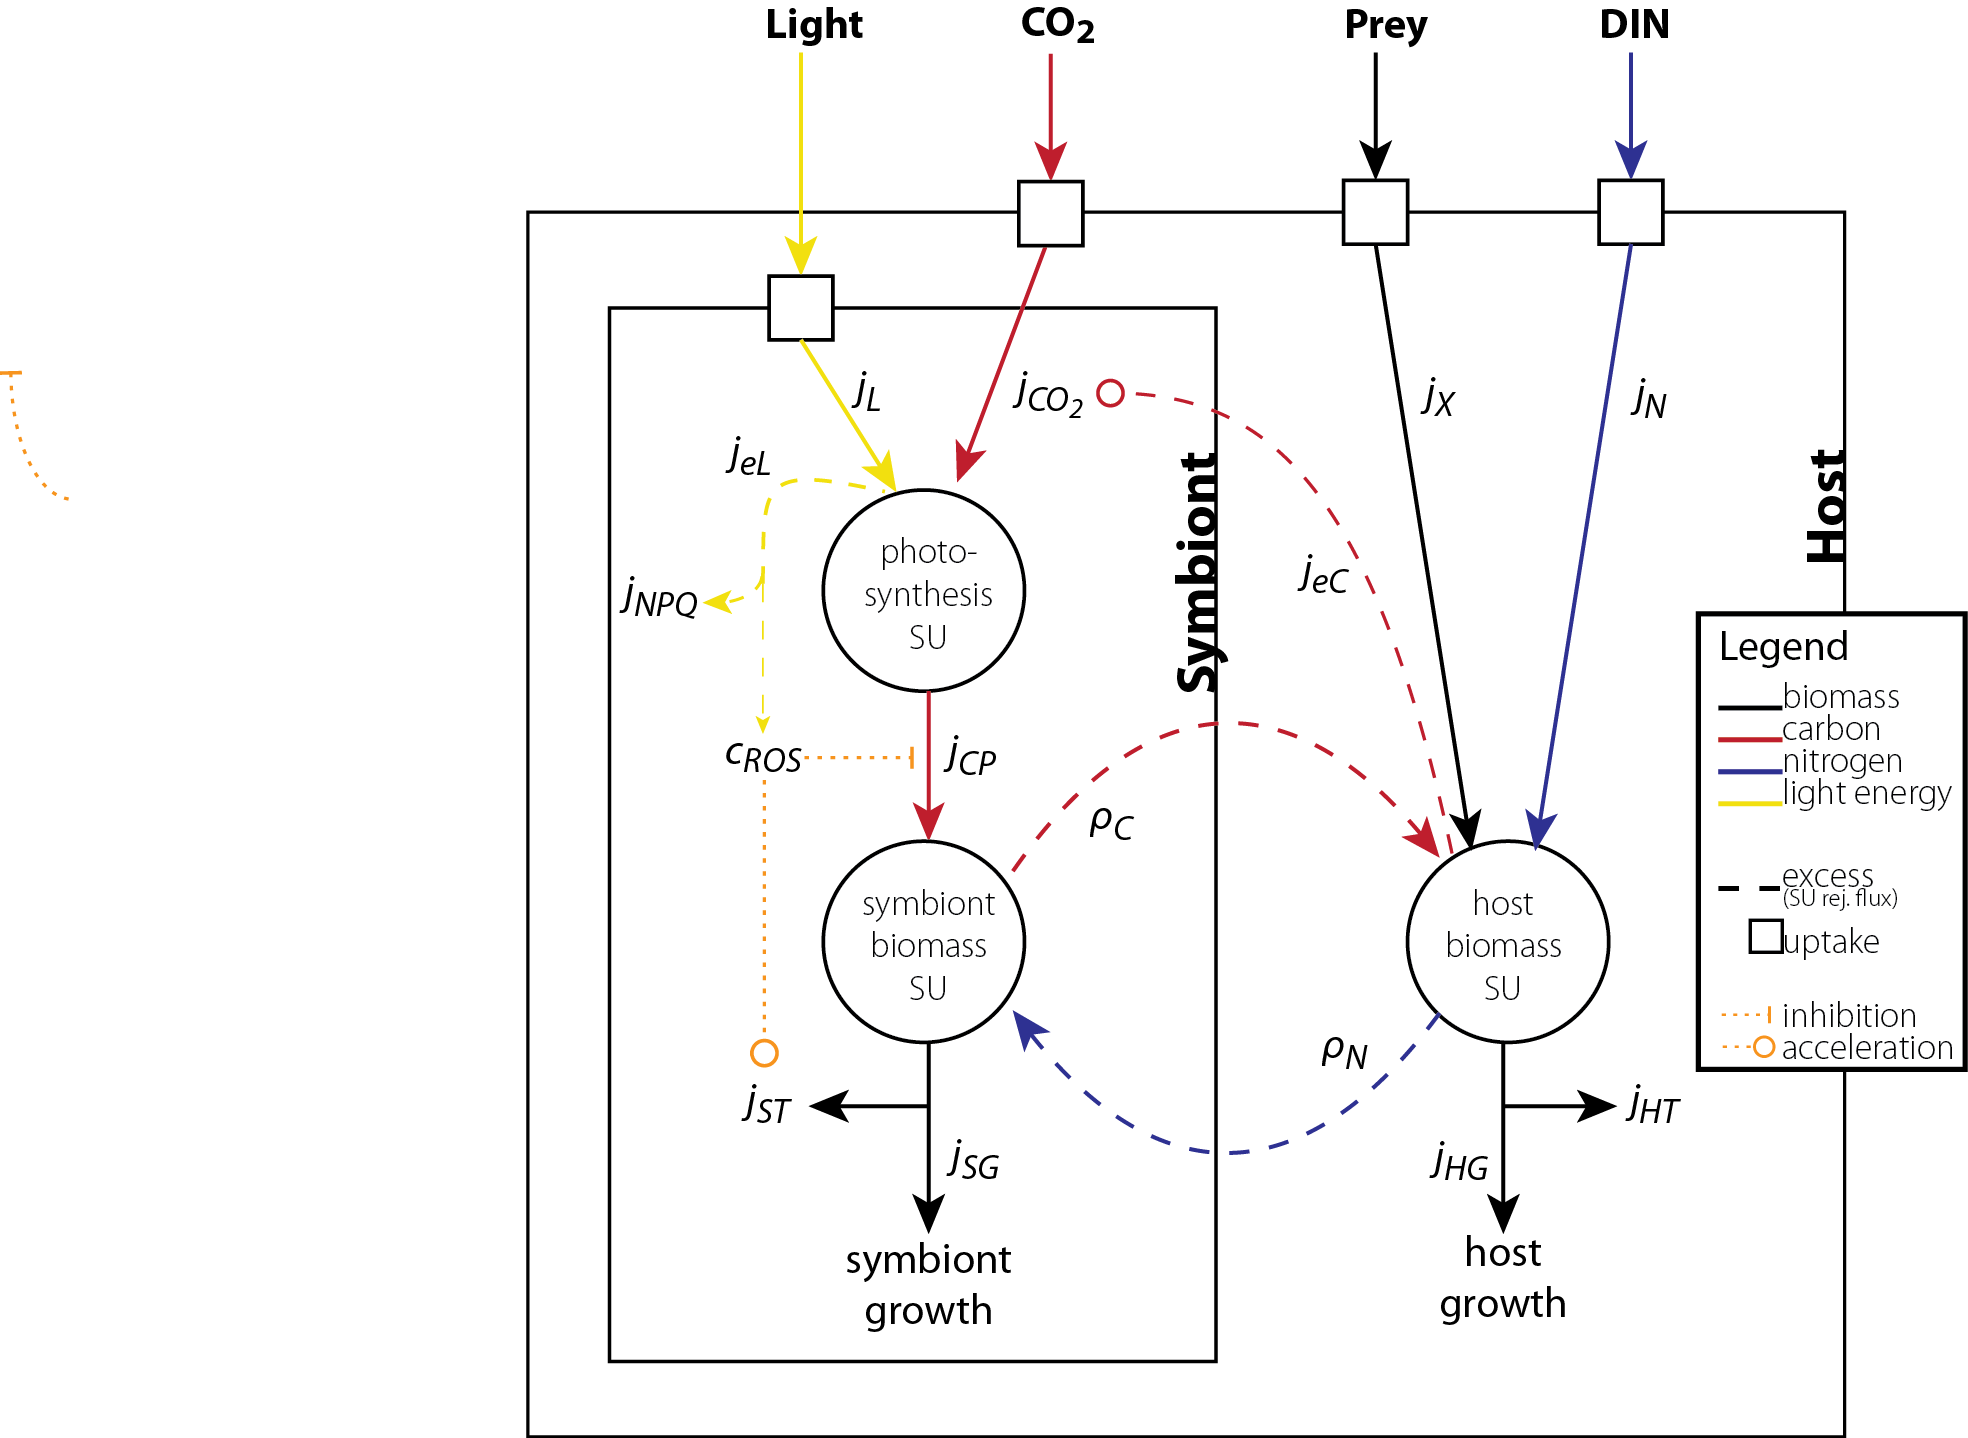
\includegraphics{../img/Fig1.png}
\caption{Graphical representation of coral-algal symbiosis model. Light,
CO\textsubscript{2}, prey, and DIN are acquired from the external
environment proportional to the biomass of the partner indicated by the
black box for uptake. Mass fluxes (see Table 1 for definitions) are
represented by \(j\)'s with subscripts indicating the type of mass, and
in some cases the process (e.g., \(j_{CP}\) is the flux of carbon
produced by photosynthesis), and \(\rho\)'s indicate fluxes that are
shared by one partner with the other. Parallel complementary
synthesizing units (SUs) are represented by large circles, and rejection
fluxes from these SUs are indicated by dashed lines. \(c_{ROS}\) is a
proportional rate that impacts other model fluxes by inhibition or
acceleration; likewise, \(j_{eC}\) accelerates the rate of \(j_{CO_2}\).
Recycling fluxes are not shown for clarity (but see Table 1 for
definitions).}
\end{figure}

\subsection{State equations}\label{state-equations}

The balance equations for symbiont (\(S\)) and host (\(H\)) biomass are
expressed as ``specific'' rates, i.e.~rates per unit of symbiont and
host biomass, respectively:

\begin{equation} {dS \over Sdt} = j_{SG} - j_{ST} \end{equation}

\begin{equation} {dH \over Hdt} = j_{HG} - j_{HT} \end{equation}

The specific biomass growth and turnover rates that define these balance
equations are produced by combinations of the individual model fluxes
(see Table 1 for definitions and units), which are each expressed as
mass-specific rates (e.g., per C-mole of symbiont or host biomass per
day). When necessary, conversions between symbiont-mass-specific and
host-mass-specific rates are accomplished by multiplying or dividing by
the symbiont:host biomass ratio.

\subsection{Coral animal fluxes}\label{coral-animal-fluxes}

The coral animal acquires both carbon and nitrogen from feeding on prey
from the environment. Assimilation from feeding is specified by
Michaelis-Menten kinetics (i.e., a Holling type II function) with a
maximum rate of \(j_{Xm}\) and half-saturation constant \(K_X\):

\begin{equation} j_X = {{j_{Xm} \cdot X} \over {X + K_X}} \end{equation}

Additionally, the coral animal acquires dissolved inorganic nitrogen
(DIN) from the surrounding seawater, which is assumed to represent
ammonium, the primary form utilized by corals (Yellowlees, Rees, and
Leggat 2008). This gives the host (rather than the symbiont) priority in
nitrogen utilization; this capacity is supported by experimental
evidence (Wang and Douglas 1998) and is consistent with the spatial
arrangment of the partners, where the host is in direct contact with the
external environment. The uptake of nitrogen from the environment is
thus specified by Michaelis-Menten kinetics using a maximum uptake rate
\(j_{Nm}\) and half-saturation constant \(K_N\):

\begin{equation} j_N = {{j_{Nm} \cdot N} \over {N + K_N}} \end{equation}

Coral biomass formation is then specified by a parallel complementary SU
(formula in Fig. 3.7 of Kooijman (2010){]}). The general form of this
equation is \((m^{-1} + x^{-1} + y^{-1} - (x + y)^{-1})^{-1}\), where
\(m\) is the maximum production flux, and \(x\) and \(y\) are the input
fluxes of the two substrates. Coral biomass is thus produced from carbon
and nitrogen according to:

\begin{equation} j_{HG} = \bigg({1 \over j_{HGm}} + {1 \over {y_{C}\rho_C{S \over H} + j_X}} + {1 \over {(j_N + n_{NX}j_X + r_{NH})n_{NH}^{-1}}} - {1 \over {y_{C}{\rho_C{S \over H} + j_X} + (j_N + n_{NX}j_X + r_{NH})n_{NH}^{-1}}}\bigg)^{-1} \end{equation}

where \(\rho_C\) is fixed carbon shared by the symbiont (see Eq. 21),
and \(r_{NH}\) is recycled nitrogen liberated by host biomass turnover
(see Eq. 7). The parameter \(y_C\) specifies the yield of biomass from
organic carbon, which we take to be 0.8 to satisfy redox balance (see
Muller et al. (2009)).

Host biomass turnover is equal to the specific maintenance rate of host
biomass,

\begin{equation} j_{HT}=j_{HT}^0 \end{equation}

and the specific flux of nitrogen that is recycled to the host biomass
SU is calcluated as:

\begin{equation} r_{NH}=\sigma_{NH}n_{NH}j_{HT} \end{equation}

The amount of nitrogen input to the coral biomass SU in excess of what
is actually consumed in biomass formation (i.e., surplus nitrogen, or
the rejection flux\footnote{Rejection fluxes must always be positive,
  and hence are specified with the notation \((x)_+\), which means
  \(max(x, 0)\).} of the SU) is then made available to the symbiont:

\begin{equation} \rho_N = (j_N + n_{NX}j_X + r_{NH} - n_{NH}j_{HG}y_{C}^{-1})_+ \end{equation}

Due to the inherent inefficiency of the parallel complementary SU
formulation, there is always some nitrogen shared with the symbiont even
when coral biomass formation is strongly nitrogen-limited. Likewise,
there is always a non-zero rejection flux of excess carbon from the
coral biomass SU. The carbon rejected from this SU reflects the amount
of excess fixed carbon available to the host that is not used in biomass
formation:

\begin{equation} j_{eC} = (j_X + \rho_C{S \over H} - j_{HG}y_{C}^{-1})_+ \end{equation}

This flux, \(j_{eC}\), is assumed to be available to the host as a
respiratory substrate to support energetically-demanding processes; of
particular importance is the host's active carbon concentrating
mechanisms (CCMs) that supply CO\textsubscript{2} for symbiont
photosynthesis (Wooldridge 2013; Hopkinson, Tansik, and Fitt 2015). We
therefore specify \(j_{CO_2}\) as the host-mediated delivery of
CO\textsubscript{2} to photosynthesis that encompasses potentially
diverse CCMs, including active transport of bicarbonate, carbonic
anhydrase-catalyzed conversion of bicarbonate to CO\textsubscript{2} to
promote diffusion toward the symbiont (Tansik, Fitt, and Hopkinson
2015), and acidification of the symbiosome to increase localized
CO\textsubscript{2} concentrations around the symbiont (Barott et al.
2014). Since these active CCMs require energetic input by the host, we
define \(j_{CO_2}\) as proportional to \(j_{eC}\), assuming that some of
this carbon is respired to energize the CCMs. This formulation means
that the symbiont indirectly ensures its own CO\textsubscript{2} supply
by providing fixed carbon (=energy) to the host (Wooldridge 2013). The
parameter \(k_{CO_2}\) scales the efficacy of host CCMs, which enables
the comparison of different rates of CO\textsubscript{2} delivery that
may characterize different coral species (Wooldridge 2014a). The active
input of CO\textsubscript{2} to the photosynthesis SU is therefore
specified as:

\begin{equation} j_{CO_2} = k_{CO_2}j_{eC} \end{equation}

\subsection{\texorpdfstring{\emph{Symbiodinium}
fluxes}{Symbiodinium fluxes}}\label{symbiodinium-fluxes}

The symbiont produces fixed carbon through photosynthesis, a process
represented here by a single SU with two substrates: light (photons) and
inorganic carbon (CO\textsubscript{2}). The amount of light absorbed by
the symbiont depends on the scalar irradiance at the site of light
absorption, which is modified substantially relative to external
downwelling irradiance owing to multiple scattering by the coral
skeleton and self-shading by surrounding symbionts (Enríquez, Méndez,
and Iglesias-Prieto 2005; Marcelino et al. 2013). We used skeletal light
amplification measurements from Marcelino et al. (2013) to empirically
derive an amplification factor, \(A\) (Figure S1), indicating the ratio
of internal scalar irradiance to external downwelling irradiance as a
function of symbiont density (S:H biomass), which is specified as:

\begin{equation} A = 1.26 + 1.39 \cdot \exp(-6.48 \cdot {S \over H}) \end{equation}

This amplification factor is then multiplied by the external downwelling
irradiance \(L\) and a parameter representing the effective
light-absorbing surface area of symbiont biomass \(\bar{a}^*\) to
specify the total light absorption:

\begin{equation} j_L =  A \cdot L \cdot \bar{a}^* \end{equation}

CO\textsubscript{2} arrives at the photosynthesis SU from multiple
sources: in addition to the CO\textsubscript{2} actively supplied by the
host through its CCMs (\(j_{CO_2}\); Eq. 10), we assume a fixed
proportion \(\sigma_{CH}\) of metabolic CO\textsubscript{2} generated by
the host from both biomass turnover and formation is passively available
to the photosynthesis SU, according to:

\begin{equation} r_{CH}=\sigma_{CH}(j_{HT} + (1-y_C)j_{HG}y_C^{-1}) \end{equation}

along with a fixed proportion of CO\textsubscript{2} generated by
symbiont biomass turnover\footnote{Note that recycling of symbiont
  biomass turnover (\(r_{NS}\) and \(r_{CS}\)) only occurs based on the
  maintenance component of turnover (i.e., \(j_{ST}^0\)), and not the
  photodamage/bleaching component, as this loss represents biomass that
  is expelled from the host.} and formation:

\begin{equation} r_{CS}=\sigma_{CS}(j_{ST}^0 + (1-y_C)j_{SG}y_C^{-1}) \end{equation}

Fixed carbon is then produced by the photosynthesis SU according to:

\begin{equation} j_{CP} = \bigg({1 \over j_{CPm}} + {1 \over {y_{CL} j_L }} + {1 \over {(j_{CO_2} + r_{CH}){H \over S} + r_{CS}}} - {1 \over {y_{CL} j_L + (j_{CO_2} + r_{CH}){H \over S} + r_{CS}}}\bigg)^{-1} \cdot c_{ROS}^{-1} \end{equation}

where \(j_{CPm}\) is the maximum specific rate of photosynthesis, and
\(c_{ROS}\) is the relative rate of reactive oxygen species production
(see Eq. 18). Dividing the photosynthetic rate by \(c_{ROS}\) causes a
decline in response to photooxidative stress at high light levels, and
the emergent outcome of this SU formulation demonstrates a classic
photoinhibition response (Fig. S2).

Light energy absorbed in excess of what is used to fix carbon is
specified by the SU rejection flux, according to:

\begin{equation} j_{eL} = (j_L - j_{CP}y_{CL}^{-1})_+ \end{equation}

This excess light energy must be quenched by alternative pathways in
order to prevent photooxidative damage (Powles 1984).
\emph{Symbiodinium} utilize a variety of pathways for non-photochemical
quenching (NPQ; Roth 2014), which we collect in a total NPQ capacity
specified as a parameter of the symbiont (\(k_{NPQ}\)). The NPQ flux
\(j_{NPQ}\) is then specified as a single-substrate SU formula with a
maximum of \(k_{NPQ}\):

\begin{equation} j_{NPQ} = (k_{NPQ}^{-1} + j_{eL}^{-1})^{-1} \end{equation}

If light energy further exceeds the capacity of both photochemistry and
NPQ, then reactive oxygen species (ROS) are produced. We represent this
as a relative quantity \(c_{ROS}\), which takes a value of 1 when all
light energy is quenched by photochemistry and NPQ, and increases as the
amount of excess excitation energy increases, specified as:

\begin{equation} c_{ROS} = 1 + {{(j_{eL} - j_{NPQ})_+} \over k_{ROS}} \end{equation}

where \(k_{ROS}\) is a parameter of the symbiont that determines the
rate of ROS production (specifically, the amount of excess excitation
energy that doubles ROS production relative to baseline levels).
Importantly, \(c_{ROS}\) is specified here not as a function of absolute
external light, but rather the amount of excess light energy after
accounting for quenching by carbon fixation and NPQ. A direct
consequence of this formulation is that CO\textsubscript{2}-limitation
of photosynthesis can lead to ROS production, an important mechanism
(Butow et al. 1998; Wooldridge 2009) that was not captured by previous
representations of photooxidative stress (Eynaud, Nisbet, and Muller
2011). With this single SU, both the light and dark reactions of
photosynthesis are represented, allowing for sink-limitation (i.e.,
CO\textsubscript{2}-limitation) to cause overreduction of the electron
transport chain and ROS production.

Carbon fixed by photosynthesis (\(j_{CP}\); Eq. 15) is then combined
with nitrogen shared by the host (\(\rho_N\); Eq. 8) and nitrogen
recycled from symbiont biomass turnover\footnote{See footnote 2.}

\begin{equation} r_{NS}=\sigma_{NS}n_{NS}j_{ST}^0 \end{equation}

to build new symbiont biomass, following the SU equation:

\begin{equation} j_{SG} = \bigg({1 \over j_{SGm}} + {1 \over y_{C}j_{CP}} + {1 \over {(\rho_N{H \over S} + r_{NS})n_{NS}^{-1}}} - {1 \over {y_{C}j_{CP} + (\rho_N{H \over S} + r_{NS})n_{NS}^{-1}}}\bigg)^{-1} \end{equation}

The rejection flux of carbon from this SU represents the amount of fixed
carbon produced by photosynthesis in excess of what can be used to
produce symbiont biomass; this surplus, \(\rho_C\), is translocated to
the coral host:

\begin{equation} \rho_C = (j_{CP} - j_{SG}y_{C}^{-1})_+ \end{equation}

Nitrogen rejected by the symbiont biomass SU, which has already been
rejected by the host biomass SU, cannot be used by either partner and is
thus lost to the environment.

Symbiont biomass turnover includes a component of constant turnover
specified by the parameter \(j_{ST}^0\), representing fixed maintenance
costs, plus a component that scales with the magnitude of ROS
production.

\begin{equation} j_{ST} = j_{ST}^0(1 + b(c_{ROS}-1)) \end{equation}

This second component of symbiont biomass loss represents both
photodamage and/or symbiont expulsion (i.e., bleaching), both of which
occur in response to high levels of ROS production. The parameter \(b\)
is included to scale biomass loss due to bleaching in response to ROS.

To aid in visualizing model results, we calculated values to indicate
the degree to which product formation at an SU was limited by
availability of either of its two substrates using the formula

\begin{equation} \log \bigg({{\min(j_{S1}, j_{Pm})} \over {\min(j_{S2}, j_{Pm})}}\bigg) \end{equation}

where \(j_{S1}\) and \(j_{S2}\) are the specific input fluxes of the two
substrates and \(j_{Pm}\) is the maximum specific product formation
rate, in units of Cmol Cmol\textsuperscript{-1} d\textsuperscript{-1}.
When both substrate input fluxes are higher than what can be used at the
maximum production rate, this limitation coefficient is zero, implying
that neither substrate is limiting production.

\subsection{Numerical analysis}\label{numerical-analysis}

The model dynamics are specified by the differential equations (1-2)
that impose biomass balance for host and symbiont and by a set of
coupled non-linear algebraic equations (3-22) that define fluxes.
Several of these fluxes are defined \emph{implicitly}; for example, the
rejection fluxes of carbon and nitrogen from the symbiont and host
biomass SUs, respectively, act as reciprocal input fluxes to the other
SU. Similarly, the photosynthesis SU receives CO\textsubscript{2} at a
rate proportional to the carbon rejection flux from the host biomass SU,
and the rejection flux of excitation energy from the photosynthesis SU
acts to reduce its own production through photoinhibition. Without
further assumptions, however, the dynamical system is not always
unambiguously defined because for some combinations of parameters and
environmental forcing functions the system of algebraic equations has
more than one solution with all fluxes non-negative (see results below).
In such circumstances, the right hand side of the differential equations
(1) and (2) is not uniquely defined even when \(S\) and \(H\) are
specified. We resolved this problem by \emph{defining the dynamical
system} as the limit as a time step \(\Delta t \rightarrow 0\) of a
discretized system corresponding to Euler integration of the
differential equations, with those fluxes that represent flows of
elemental matter implemented by assuming that transfer of material
between components of the system takes one time step. Thus, for example,
CO\textsubscript{2} rejected from the host SU at time \(t\) arrives at
the photosynthesis SU at time \(t + \Delta t\).

Simulations using the discretized scheme were performed using R code
developed in the coRal R package \url{github.com/jrcunning/coRal}. By
experimentation, we found that a time step of 0.1 days gave adequate
precision for most simulations (including used to generate Figs. 2-8 in
this paper). For steady state estimations, simulations were run until
the changes in specific growth rate of the host and the S:H biomass
ratio were less than 1e-5 per time step. In regions of state space where
very slow transient dynamics could be expected (i.e.~near bifurcation
points), sample steady state calculations were verified using
MATHEMATICA code for numerical root finding (function FindRoot) with the
code written independently by a coauthor without reference to the R
code. All of the R code for the simulations and figures presented in
this paper can be found in the accompanying data repository at
\url{github.com/jrcunning/coRal-analysis}.

\section{Steady state behavior}\label{steady-state-behavior}

In a constant environment, the system ultimately reaches a steady state
of exponential growth or decline. However, under some conditions, either
of these outcomes may occur depending on initial values of symbiont and
host biomass, indicating the presence of alternate stable states (Fig.
2). The mechanism that produces these alternate stable states is the
positive feedback between carbon-limitation of the host and
CO\textsubscript{2}-limitation of photosynthesis: if symbiont biomass is
initially very low (i.e., a ``bleached'' coral), very little carbon is
fixed, and the system cannot escape this positive feedback and cannot
grow (unless feeding is sufficiently high). However, if symbiont biomass
is initially high (i.e., a ``healthy'' coral), then the system remains
in a nitrogen-limited state with positive growth. For practical
purposes, this section of the manuscript considers only positive growth
steady states under constant environments; subsequently, we explore how
environmental forcing may cause the system to switch between alternate
stable states, which we interpret in the context of coral bleaching (see
``Coral Bleaching and Recovery'', below).

\begin{figure}[htbp]
\centering
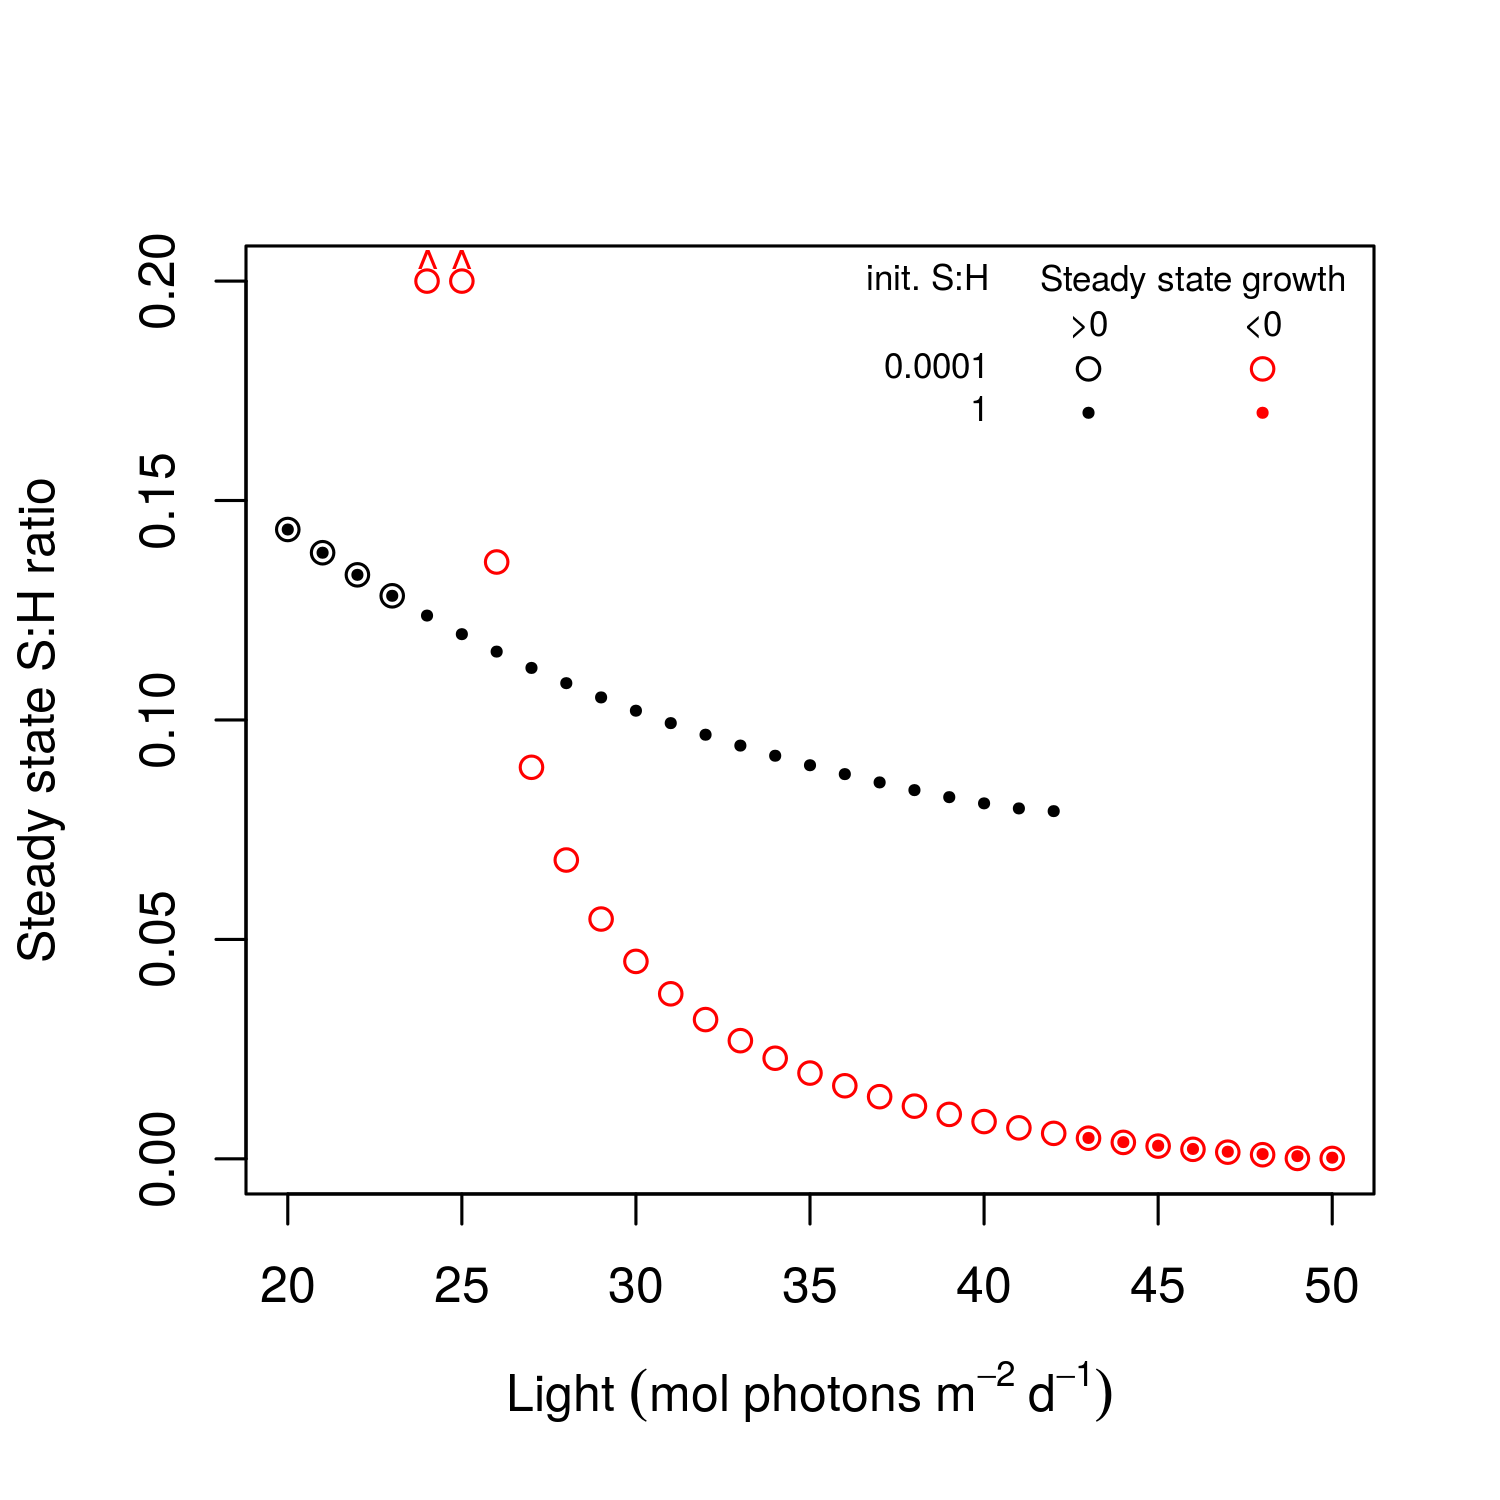
\includegraphics{../img/Fig2.png}
\caption{Alternate stable states in S:H biomass and growth across a
light gradient. Alternate stable states occur between
\textasciitilde{}25-42 mol photons m\textsuperscript{-2}
d\textsuperscript{-1} under these conditions (DIN=1e-7 mol N
L\textsuperscript{-1}; X=1e-7 C-mol X L\textsuperscript{-1}), depending
on whether initial S:H is high (1, closed circles), representing a
healthy coral, or low (0.0001, open circles), representing a bleached
coral. Arrow above point at L=25 indicates a S:H ratio beyond the axis
range; this `overshoot' phenomenon, in which initially bleached corals
may achieve high S:H ratios while remaining in a carbon-limited state is
discussed in the \emph{Coral Bleaching and Recovery} section.}
\end{figure}

To analyze positive-growth steady state behavior, we ran the model to
steady state across gradients of external irradiance and nutrients (Fig.
3), which revealed patterns consistent with observed phenomena in
corals. Predicted growth rates are low at low light and DIN
(\textasciitilde{}0.01 d\textsuperscript{-1}), and begin increasing as
both of these factors increase (Fig. 3A). Low light limits
photosynthetic rates, resulting in less fixed carbon shared with the
host and an associated increase in the symbiont to host biomass ratio
(Fig. 3B). In agreement with this trend are many observations of
negative correlation between irradiance and symbiont density (Stimson
1997; Brown et al. 1999; Fitt et al. 2000; Titlyanov et al. 2001). As
higher light alleviates light-limitation of photosynthesis, host growth
becomes less carbon-limited.

\begin{figure}[htbp]
\centering
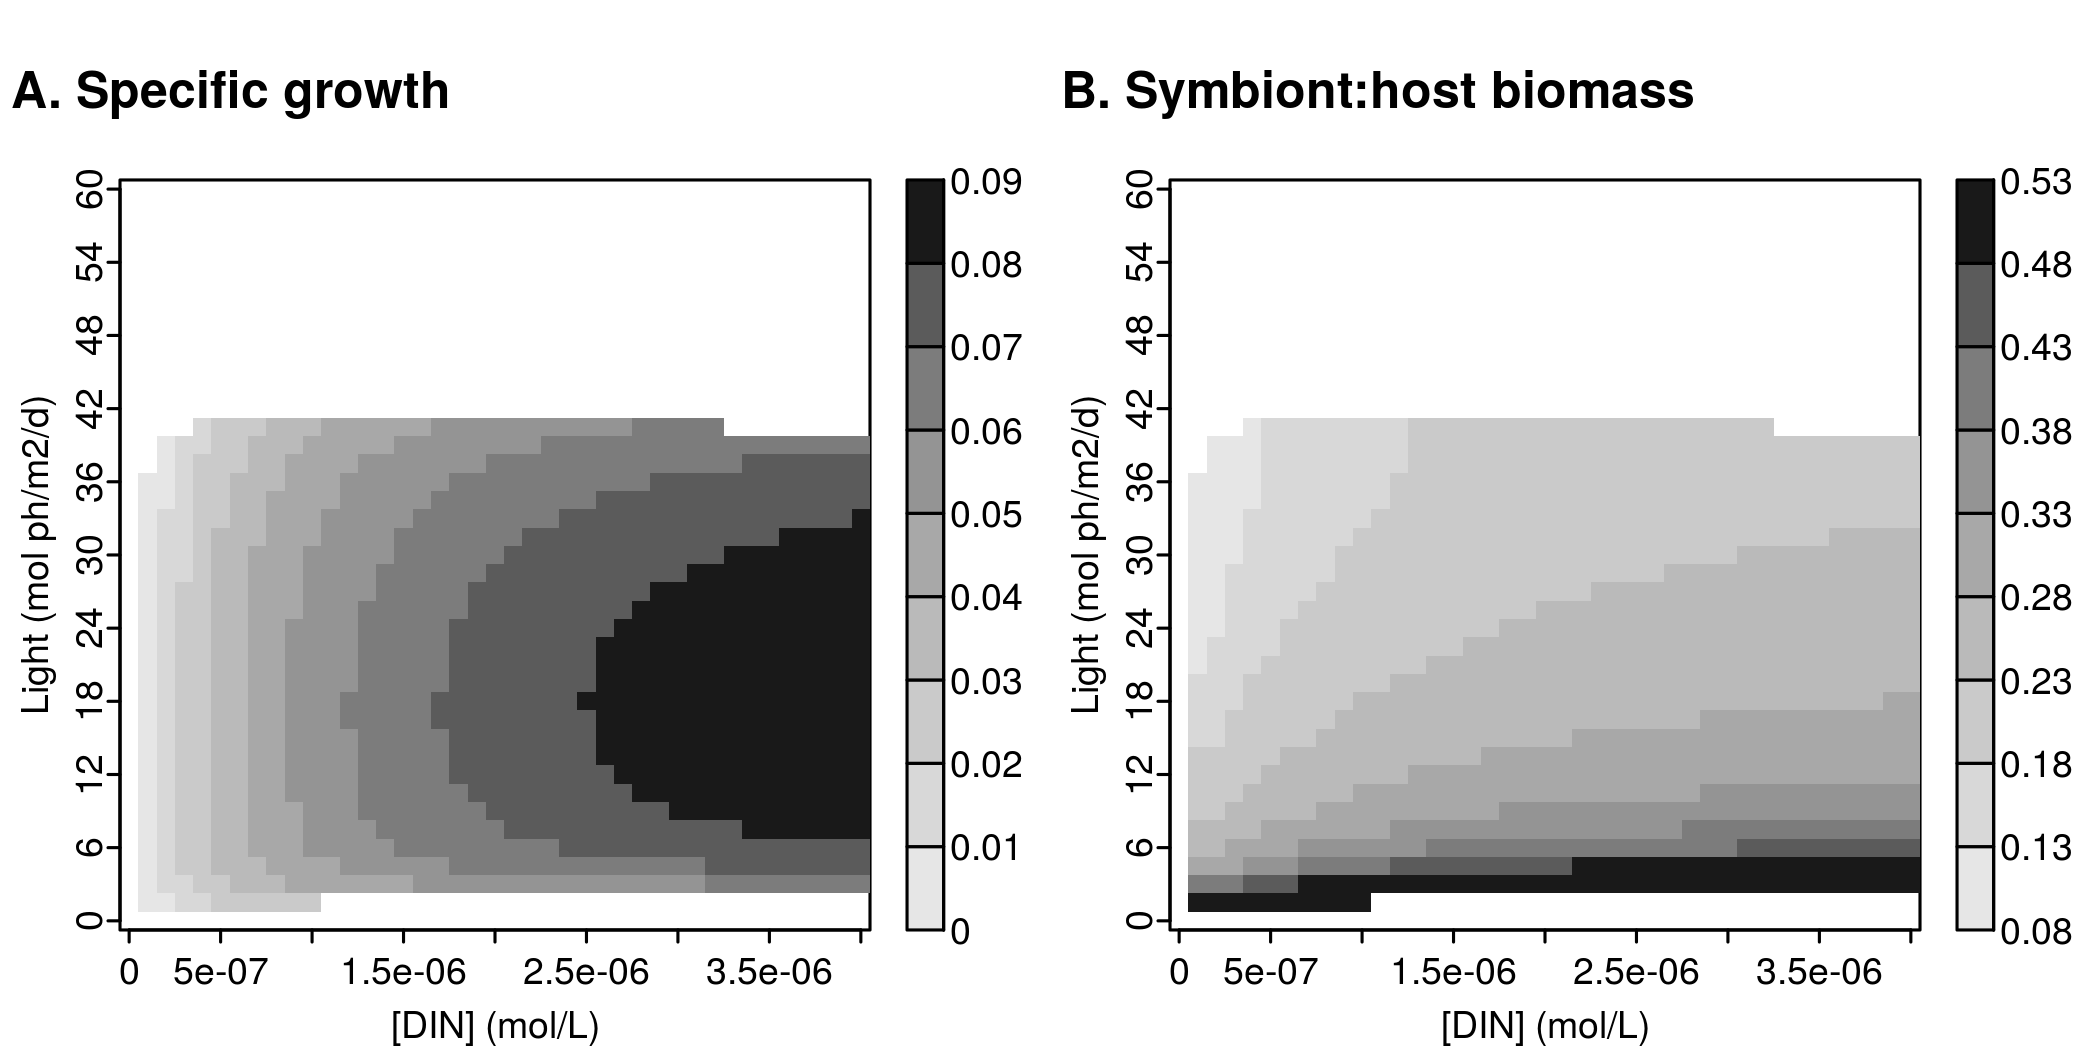
\includegraphics{../img/Fig3.png}
\caption{Steady state values of (A) specific growth (C-mol H C-mol
H\textsuperscript{-1} d\textsuperscript{-1}) and (B) the symbiont to
host biomass ratio (C-mol S C-mol H\textsuperscript{-1}) across
gradients of external irradiance and dissolved inorganic nitrogen. Note
that typical conditions for reefs are \textasciitilde{}1e-7 M DIN and
10-20 mol photons m\textsuperscript{-2} d\textsuperscript{-1}.
Simulations for each combination of light and nutrients (41 points along
each axis) were run to steady state with all parameters at default
values and prey density set to zero. Negative steady state growth rates
and corresponding S:H ratios were set to zero, and a ceiling of 0.5 was
imposed on S:H ratios to aid in visualization.}
\end{figure}

Similarly, increasing DIN alleviates nitrogen-limitation (Fig. 3A).
Increased growth at higher DIN is predicted by the DEB model of Muller
et al. (2009), and has also been observed experimentally (Muller-Parker
et al. 1994; Tanaka et al. 2007; Tanaka et al. 2013). However, DIN
elevation beyond a certain point (e.g., \textasciitilde{}3-4 µM in these
simulations) has little effect on growth as carbon becomes limiting.
Although very high nutrient levels may reduce growth in nature (Shantz,
Lemoine, and Burkepile 2015), these impacts are not likely to occur
within the range of concentrations considered here (\textless{}4 µM)
(Ferrier-Pagès et al. 2000). In addition to increasing growth, DIN also
increases the symbiont to host biomass ratio (Fig. 3B), a phenomenon
also observed in reef corals (Marubini and Davies 1996). At low DIN and
intermediate light, more typical of coral reef environments, symbiont to
host biomass ratios are around \textasciitilde{}0.06-0.21, which is
consistent with values reported in the literature (Muscatine, R
McCloskey, and E Marian 1981; Edmunds et al. 2011; Hawkins et al. 2016).

The maximum predicted growth rates of \textasciitilde{}0.1
d\textsuperscript{-1}, occurring between \textasciitilde{}10-25 mol
photons m\textsuperscript{-2} d\textsuperscript{-1} light and
\textasciitilde{}4 µM DIN (Fig. 3A), are comparable to the rate of 0.07
d\textsuperscript{-1} measured by Tanaka et al. (2007) in \emph{Acropora
pulchra} under similar N-enriched conditions. Under conditions more
typical of reef environments (\textless{}0.5 µM DIN), predicted growth
rates are \textasciitilde{}0.01-0.03 d\textsuperscript{-1}. Observed
specific growth rates in several coral species fall near or below the
lower end of this range (\textasciitilde{}0.01 d\textsuperscript{-1})
(Osinga et al. 2011; Osinga et al. 2012), though values as high as 0.025
d\textsuperscript{-1} have been reported in \emph{Galaxea fascicularis}
(Schutter et al. 2010), and 0.04 d\textsuperscript{-1} in \emph{Aiptasia
diaphana}, a non-calcifying symbiotic anemone (Armoza-Zvuloni et al.
2014). However, it is not surprising that observed growth rates are
often lower than model predictions, since the model does not account for
ecological factors that may limit growth (e.g., competition, predation,
bioerosion). Furthermore, while most measurements are made on skeletal
growth, the model predicts biomass growth, which may not always be
strongly correlated (Anthony 2002).

At irradiance levels above \textasciitilde{}25 mol photons
m\textsuperscript{-2} d\textsuperscript{-1}, steady state growth rates
decline until positive growth ceases above \textasciitilde{}40 µmol
photons m\textsuperscript{-2} d\textsuperscript{-1} (Fig. 3A). The
mechanism underlying this decline is the increase in light energy beyond
the capacities of photosynthesis and non-photochemical quenching: excess
excitation energy generates reactive oxygen species (ROS) (Weis 2008;
Roth 2014), which, in this model, have the phenomenological consequences
of reducing the photosynthetic rate (representing photoinhibition) and
increasing symbiont biomass loss (representing photodamage and/or
symbiont expulsion) (see Eynaud, Nisbet, and Muller 2011). Together,
these impacts reduce the symbiont to host biomass ratio (Fig. 3B), as
occurs during coral bleaching. This reduction in symbionts consequently
reduces the flux of fixed carbon to the host, resulting in increasing
carbon-limitation (Fig. 3B) and eventual cessation of growth (Fig. 3A).

The incorporation of photooxidative stress in the model sets an upper
limit to the amount of light at which a stable symbiotic interaction can
be maintained, but even below this threshold of breakdown, negative
effects of high light reduce steady state growth and symbiont:host
biomass (Fig. 3). This gradual decline is consistent with experimental
results showing that high light levels decrease growth (Schutter et al.
2011), and field studies documenting optimum growth rates at
intermediate depths (Baker and Weber 1975; Huston 1985). By
incorporating these impacts of light stress, the model predicts greater,
and more realistic, variation in state variables across light gradients
than was predicted by the models of Muller et al. (2009), which did not
include photoinhibition or photodamage, or Eynaud, Nisbet, and Muller
(2011), which included representations of photoinhibition or photodamage
separately. It is important to recognize that the upper light limit set
by photooxidative stress on a stable symbiosis under steady state
conditions (Fig. 3) may be temporarily crossed by a dynamic system,
which may experience a period of symbiont loss (bleaching) and reduced
growth, after which a return to benign conditions may restore symbiont
biomass and positive growth. To explore this further and illustrate the
behavior of the model in more detail, we evaluate a number of dynamic
simulations below (see ``Dynamic behavior'').

\section{Sensitivity analysis}\label{sensitivity-analysis}

The values used for each parameter in the model (Table 2) are derived
from relevant literature (see Supplementary Information). Here we
evaluate the sensitivity of the model to changes in these parameter
values, which also serves to demonstrate the behavior of the dynamical
system. We calculated fractional change in steady state values in
response to fractional changes in parameter values, relative to their
default values, under environmental conditions typical of coral reefs.

\begin{figure}[htbp]
\centering
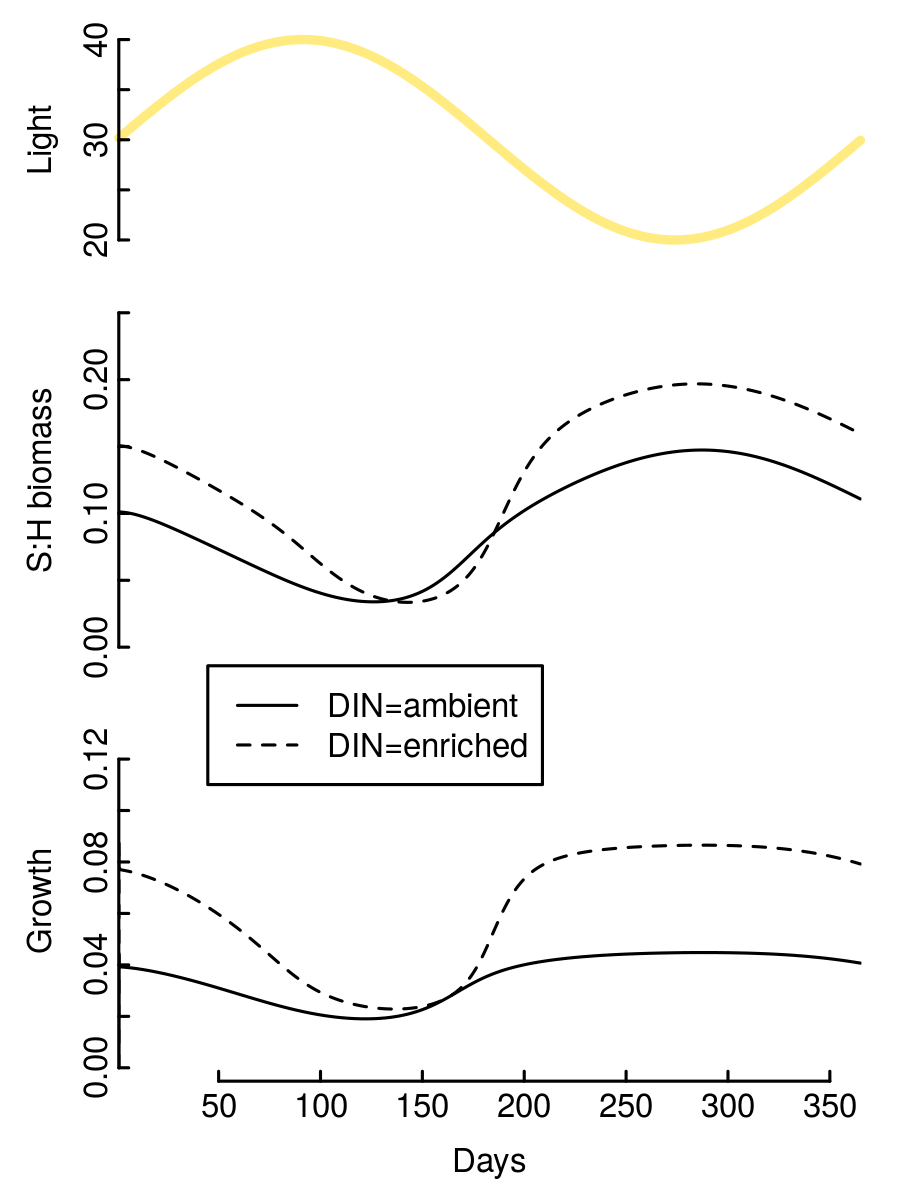
\includegraphics{../img/Fig4.png}
\caption{Sensitivity analysis. Plots show the fractional change in
steady state values of growth rate (solid lines) and S:H biomass (dashed
lines) in response to fractional changes in default parameter values
(see Table 2 for default values). Parameters are grouped by the
processes in which they are involved. This sensitivity analysis was
conducted at conditions typical for coral reef environments: low DIN
(1e-7 M) and intermediate light (15 mol photons m\textsuperscript{-2}
d\textsuperscript{-2}), with prey density set to zero. Sensitivity
analyses conducted other environmental conditions are presented in Figs
S3-S7.}
\end{figure}

Overall, relative changes in the steady state of the system are less
than the equivalent relative change in parameter value. However, changes
in certain parameter values have more significant impacts: increasing
\(j_{Nm}\) or decreasing \(K_N\) both dramatically increase host growth
(Fig. 4), demonstrating the strong nitrogen-limitation that
characterizes these symbioses. The parameter \(\bar{a}^*\) has a strong
impact on S:H biomass ratios (Fig. 4) since this parameter determines
the amount of light absorbed by symbionts, with lower values increasing
light-limitation. Increasing the maximum growth and turnover rates have
the expected effects of increasing and decreasing growth, respectively.
Parameters relating to photooxidative stress and bleaching have little
impact under low nutrients and intermediate light (Fig. 4), but have
larger impacts under higher light (e.g., Fig. S6). Sensitivity analyses
conducted under different combinations of external light and nutrients
are presented in Figs. S3-S7.

\section{Dynamic behavior}\label{dynamic-behavior}

The dynamic behavior of the model demonstrates its power to integrate
multiple environmental forcings simultaneously. Here we present several
scenarios that demonstrate the model's ability to reproduce complex
phenomena that have been observed in corals.

\subsection{Seasonal variability}\label{seasonal-variability}

Symbiont densities and coral growth rates are known to vary seasonally,
representing an integrated response to changes in a suite of
environmental factors. Light in particular is a strong driver of these
trends (Stimson 1997; Brown et al. 1999; Fagoonee et al. 1999; Fitt et
al. 2000), with high light associated with lower symbiont abundance and
reduced tissue biomass. The role of light in driving seasonal changes in
symbiont density was demonstrated nicely by Stimson (1997), who also
found that experimental nutrient-enrichment amplified the light-driven
seasonal oscillation. Using the levels of light and nutrients from this
study as inputs, the model reproduces this observed interaction among
environmental factors (Fig. 5), and also provides the mechanism:
increasing light in summer decreases symbiont growth rates due to
photooxidative stress, leading to decreasing S:H ratios. Under nutrient
enrichment, this effect is more pronounced, as
CO\textsubscript{2}-limitation of photosynthesis (due to higher symbiont
standing stocks) causes mild bleaching that results in a similar
summertime minimum S:H as the ambient nutrient case (`physiological
bleaching' \emph{sensu} Fitt et al. (2001)). Decreasing light into
winter then alleviates the photooxidative stress constraints on carbon
fixation such that nitrogen-limitation constrains the S:H ratio,
explaining why S:H increases more when DIN is enriched (Fig. S8).

\begin{figure}[htbp]
\centering
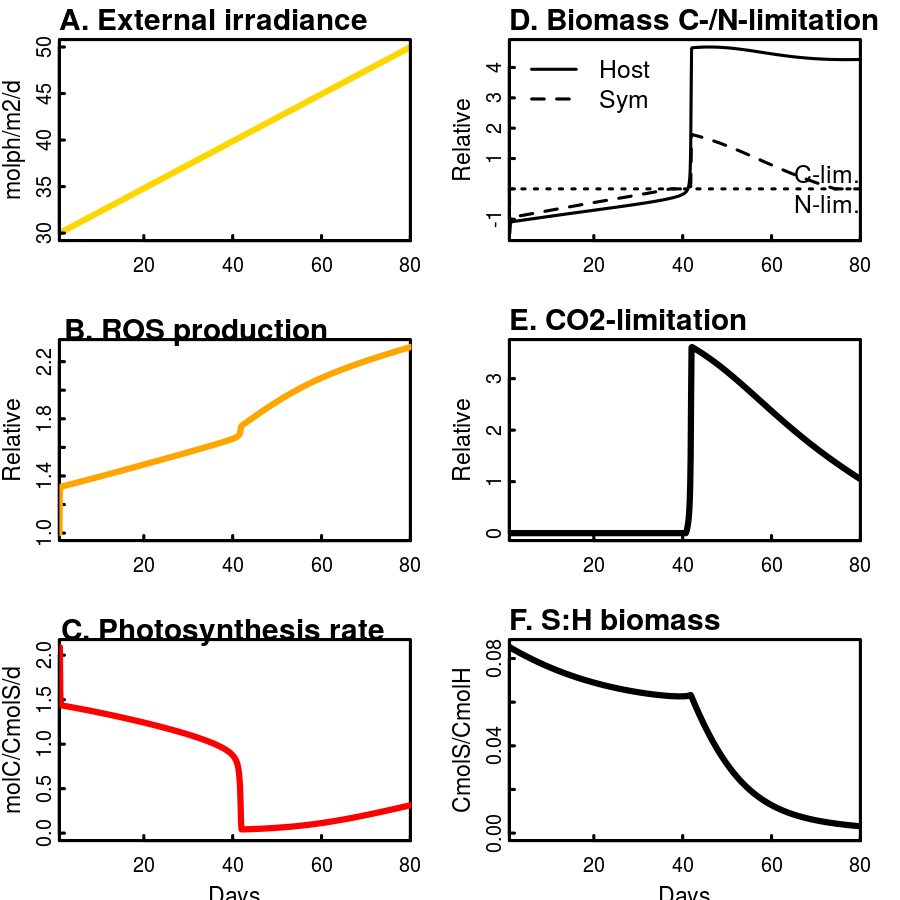
\includegraphics{../img/Fig5.png}
\caption{Light-driven seasonal dynamics of symbiont abundance and coral
growth. Light input (upper panel) was designed as a sinusoidal curve
with a period of one year, with maximum and minimum values of 44 and 20
mol photons m\textsuperscript{-2} d\textsuperscript{-1}, corresponding
to those measured by Stimson (1997). The dynamic behavior of symbiont to
host biomass ratio (middle panel) and the specific growth rate of host
biomass (lower panel) show seasonal oscillations that are greater in
magnitude under high nutrients (15.14 \(\mu\)M N; dashed lines) relative
to low nutrients (0.14 \(\mu\)M N; solid lines), consistent with the
findings of Stimson (1997). Prey density was set at 1e-6 CmolX
L\textsuperscript{-1}.}
\end{figure}

The prediction of higher growth when light is reduced indicates that
growth is not limited by low light in winter, but is actually reduced by
excess light in summer\footnote{at the light levels indicated in Stimson
  (1997). Note that if light levels were reduced throughout the year
  (e.g.~for a coral at greater depth) such that light did not cause
  photo-oxidative stress in summer but became limiting to photosynthesis
  in winter, the S:H ratio would still increase in winter, but growth
  would decrease; the latter scenario is predicted both by the present
  model as well as that of Muller et al. (2009), since photo-oxidative
  stress does not become relevant.}, consistent with the experimental
findings of Schutter et al. (2011). Seasonal summertime reductions in
tissue biomass have also been well-documented in the field (Fitt et al.
2000), along with reductions in net photosynthetic capacity
(Muller-Parker 1987). Importantly, while light alone may drive seasonal
dynamics in the ways discussed\footnote{See footnote 4.}, temperature
fluctuations may attenuate or even reverse the effect of light as cooler
winters depress metabolism. Seasonal changes in nutrients associated
with fertilization use and runoff during growing seasons may also impact
these dynamics. Thus, the relative magnitude of fluctuation in
temperature, light, and nutrients may produce wide variability in the
direction and magnitude of seasonal changes in growth and symbiont
abundance, depending on location and microhabitat. Nevertheless, the
seasonal variability predicted here in response to light (Fig. 5) is
consistent with experimental and field observations for corals, and
demonstrates the model's ability to predict dynamic behavior that
mechanistically integrates multiple environmental drivers.

\subsection{Coral bleaching and
recovery}\label{coral-bleaching-and-recovery}

Coral bleaching is the stress-induced loss of symbiotic algae from coral
tissues, which can occur in response to a variety of environmental
stressors. In most cases, coral bleaching is thought to begin with
photooxidative stress in symbiont photosynthesis (Lesser 1997), which
triggers a cascade of events leading to symbiont expulsion (Weis 2008).
As symbionts are expelled, the host receives less fixed carbon, which
may then compromise its ability to activate CCMs that deliver
CO\textsubscript{2} to photosynthesis (Wooldridge 2013). Increasing
CO\textsubscript{2}-limitation for remaining symbionts, along with an
amplified internal light environment due to reduced self-shading
(Enríquez, Méndez, and Iglesias-Prieto 2005), may further exacerbate
photooxidative stress and accelerate symbiont expulsion, driving the
coral into a bleached state.

While these positive feedbacks have been discussed previously in the
literature, this is the first attempt to implement and explore their
properties within a dynamical model. Interestingly, these feedbacks lead
to alternate stable states in the symbiotic system. The `healthy' state
is characterized by nitrogen-limitation of both symbiont and host: under
these conditions, the symbiont translocates sufficient carbon to support
host growth and CCMs, which ensures that photosynthesis does not become
CO\textsubscript{2}-limited. However, if carbon translocation is
disrupted (and light is sufficiently high), then the system is driven
into the `bleached' state by photooxidative stress and positively
reinforcing carbon- and CO\textsubscript{2}-limitation. In this context,
coral bleaching can be understood as a transition from one stable state
to another, and bleaching thresholds are sets of environmental
conditions that push a healthy-state coral onto a trajectory leading to
a bleached state.

We are highly interested in the conditions under which the system
switches from a healthy to a bleached state, and can use this model as a
tool to explore this dynamic behavior. Most straightforwardly, this
switch occurs when increasing external irradiance (Fig. 6A) causes
sufficient ROS production (Fig. 6B) and photoinhibition (Fig. 6C) that
the positive feedbacks between host carbon-limitation (Fig. 6D) and
CO\textsubscript{2}-limitation of photosynthesis (Fig. 6E) are rapidly
engaged, leading to even greater photooxidative stress and a rapid
decline in S:H biomass (Fig. 6F), characteristic of coral bleaching.
However, the positive feedbacks involved in bleaching are not engaged
only in response to high external irradiance alone; in fact, they depend
on the relative balance of light energy absorption and quenching, which
in turn depends on the availability of CO\textsubscript{2} for
photosynthesis. While previous models framed photooxidative stress as a
fixed response to absolute external irradiance (Eynaud, Nisbet, and
Muller 2011), our implementation considers the dynamic balance of
multiple energy sinks in the causation of stress, which is more
consistent with current understanding of symbiosis dysfunction
(Wooldridge 2013), and establishes a critical role of host CCMs in
providing CO\textsubscript{2} for photosynthesis (Tansik, Fitt, and
Hopkinson 2015; Hopkinson, Tansik, and Fitt 2015).

\begin{figure}[htbp]
\centering
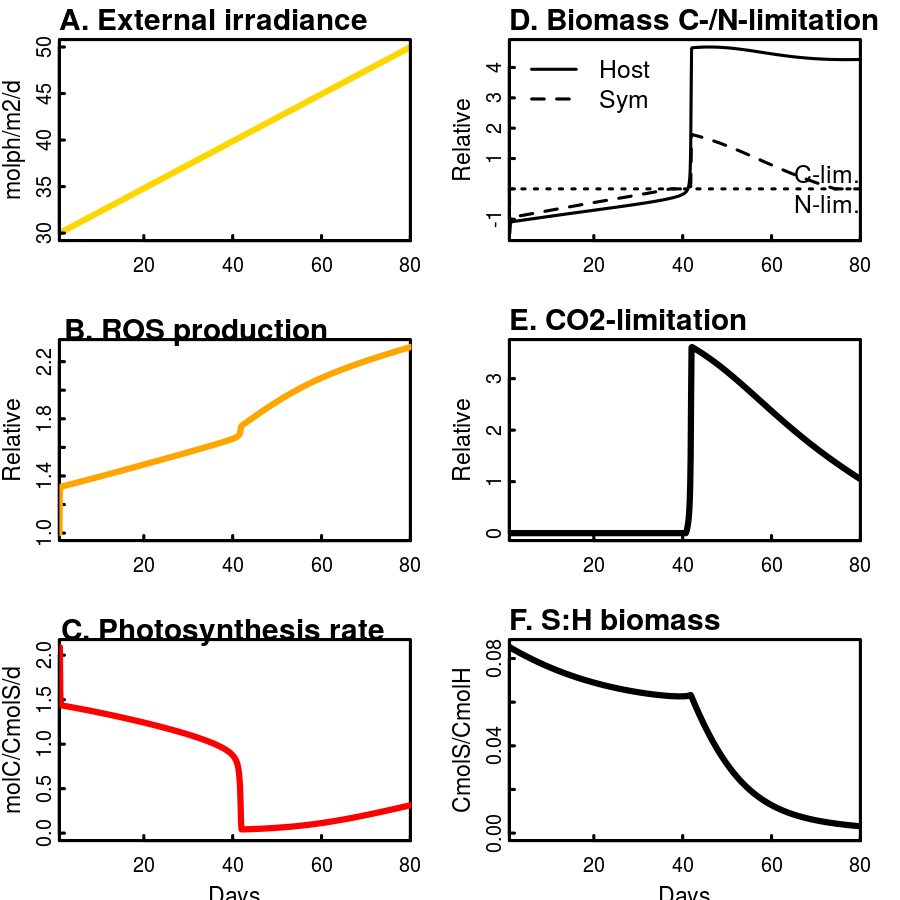
\includegraphics{../img/Fig6.png}
\caption{Coral bleaching as a switch from a nitrogen- to carbon-limited
alternative stable state. This transition is demonstrated in response to
gradually increasing external light (A), which causes an increase in
production of ROS (B) that reduces the photosynthetic rate through
photoinhibition (C). Decreasing photosynthesis moves the system from
overall nitrogen-limitation toward carbon-limitation (D); when this
threshold is crossed, the system rapidly becomes highly carbon-limited
as photosynthesis becomes CO\textsubscript{2}-limited (E) and symbiont
densities rapidly decline (F) into a bleached state. Substrate
limitation coefficients were calculated using Eq. 23. All parameters
were set at default values with external DIN=1e-7 mol N/L and prey
density set to zero).}
\end{figure}

The importance of host CCM activity establishes significant interactive
roles for other factors in influencing coral bleaching responses. For
example, simulations of high light stress (Fig. 7) demonstrate that
bleaching can be attenuated by heterotrophic feeding, a phenomenon which
has been observed experimentally (Borell et al. 2008). The mechanism
underlying this prediction is that feeding by the host increases host
CCM activity, which delays the onset of CO\textsubscript{2}-limitation
of photosynthesis and reduces bleaching severity. On the other hand,
elevated nutrients exacerbate bleaching (Fig. 7), since higher symbiont
densities are more susceptible to CO\textsubscript{2}-limitation
(Wooldridge 2009). Several experimental (Wiedenmann et al. 2013; Cunning
and Baker 2013; Vega Thurber et al. 2014) and correlational studies
(Wooldridge and Done 2009) are consistent with this mechanistic link
between high nutrients and bleaching.

\begin{figure}[htbp]
\centering
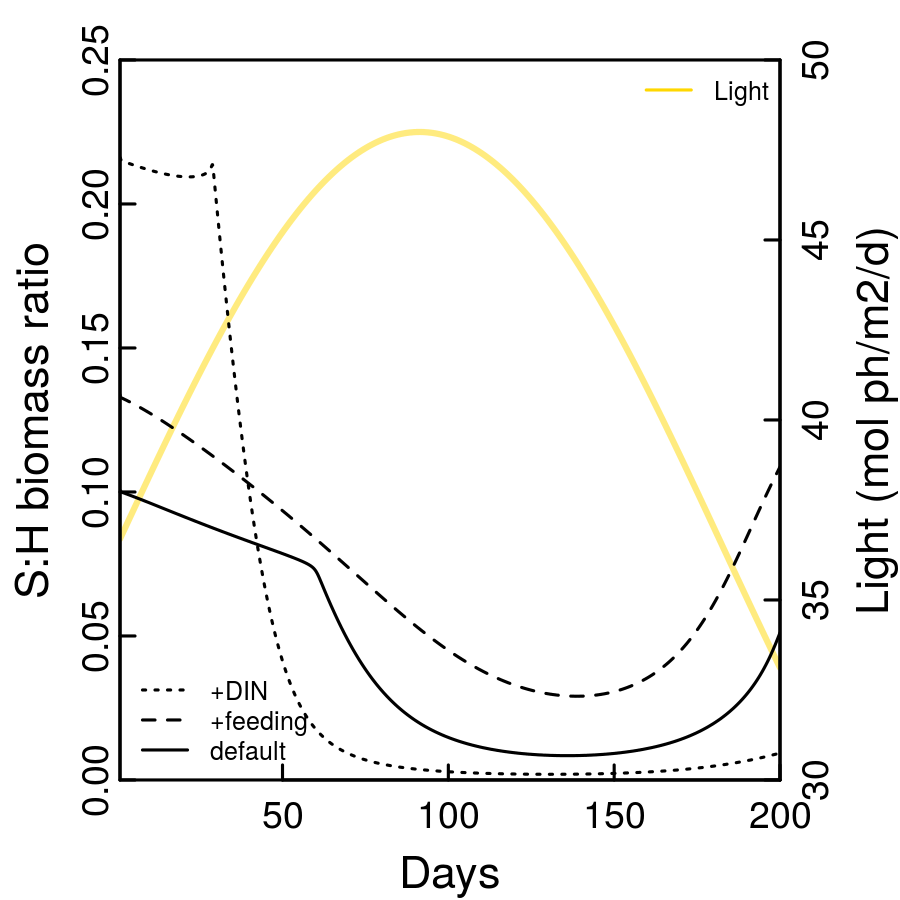
\includegraphics{../img/Fig7.png}
\caption{Bleaching with interactive factors. Simulations of high light
stress (sinusoid with maximum=48 mol ph m\textsuperscript{-2}
d\textsuperscript{-1}) under default environmental conditions (solid
line; DIN=1e-7 mol N L\textsuperscript{-1}; prey=2e-7 C-molX
L\textsuperscript{-1}), or with elevated feeding (dashed line; prey=1e-6
C-molX L\textsuperscript{-1}), or elevated nutrients (dotted line;
DIN=4e-6 mol N L\textsuperscript{-1}). Initial symbiont biomass was set
to the steady state for each set of starting conditions, with all other
parameters at default values.}
\end{figure}

Since bleaching can be understood as a transition from a
nitrogen-limited state with high S:H biomass to a carbon-limited state
with low S:H biomass, induced by an external stressor, recovery can be
understood as a switch back to the nitrogen-limited state once the
external stressor is alleviated. In natural settings, this typically
occurs through seasonal declines in temperature and light. However,
hysteresis associated with the system's alternate stable states
indicates that the symbiosis cannot recover along the same trajectory it
followed during bleaching; indeed, the stressor must be alleviated
\emph{below} the threshold that initially caused bleaching in order for
the system to recover (Fig. 2). This is because under the same external
conditions, a bleached coral with low S:H biomass (relative to a healthy
coral with high S:H biomass) is characterized by greater light
amplification and weaker CCM activity, which enhance photooxidative
stress and serve to maintain the carbon-limited state. In order for the
system to recover, the stressor must be reduced enough such that
photooxidative stress ceases and translocation of carbon from symbiont
to host is resumed. Once this occurs, the host can energize its CCMs,
which further enhances carbon fixation and accelerates the system back
toward a nitrogen-limited state, indicative of recovery. The conditions
under which recovery can occur -- which determine the magnitude of
hysteresis (Fig. 8) -- depend on the relative abundance of nitrogen and
carbon in the environment. Higher food levels, representing a
non-autotrophic carbon source for the host, make it easier for the host
to overcome carbon-limitation (Fig. 8A, D), thus providing a potential
mechanism underlying observations that feeding aids recovery from
bleaching (Grottoli, Rodrigues, and Palardy 2006; Connolly,
Lopez-Yglesias, and Anthony 2012). Conversely, high external DIN impedes
the re-establishment of nitrogen-limitation, making recovery from
bleaching more difficult (i.e., narrowing - or eliminating - conditions
under which recovery is possible, Fig. 8C).

\begin{figure}[htbp]
\centering
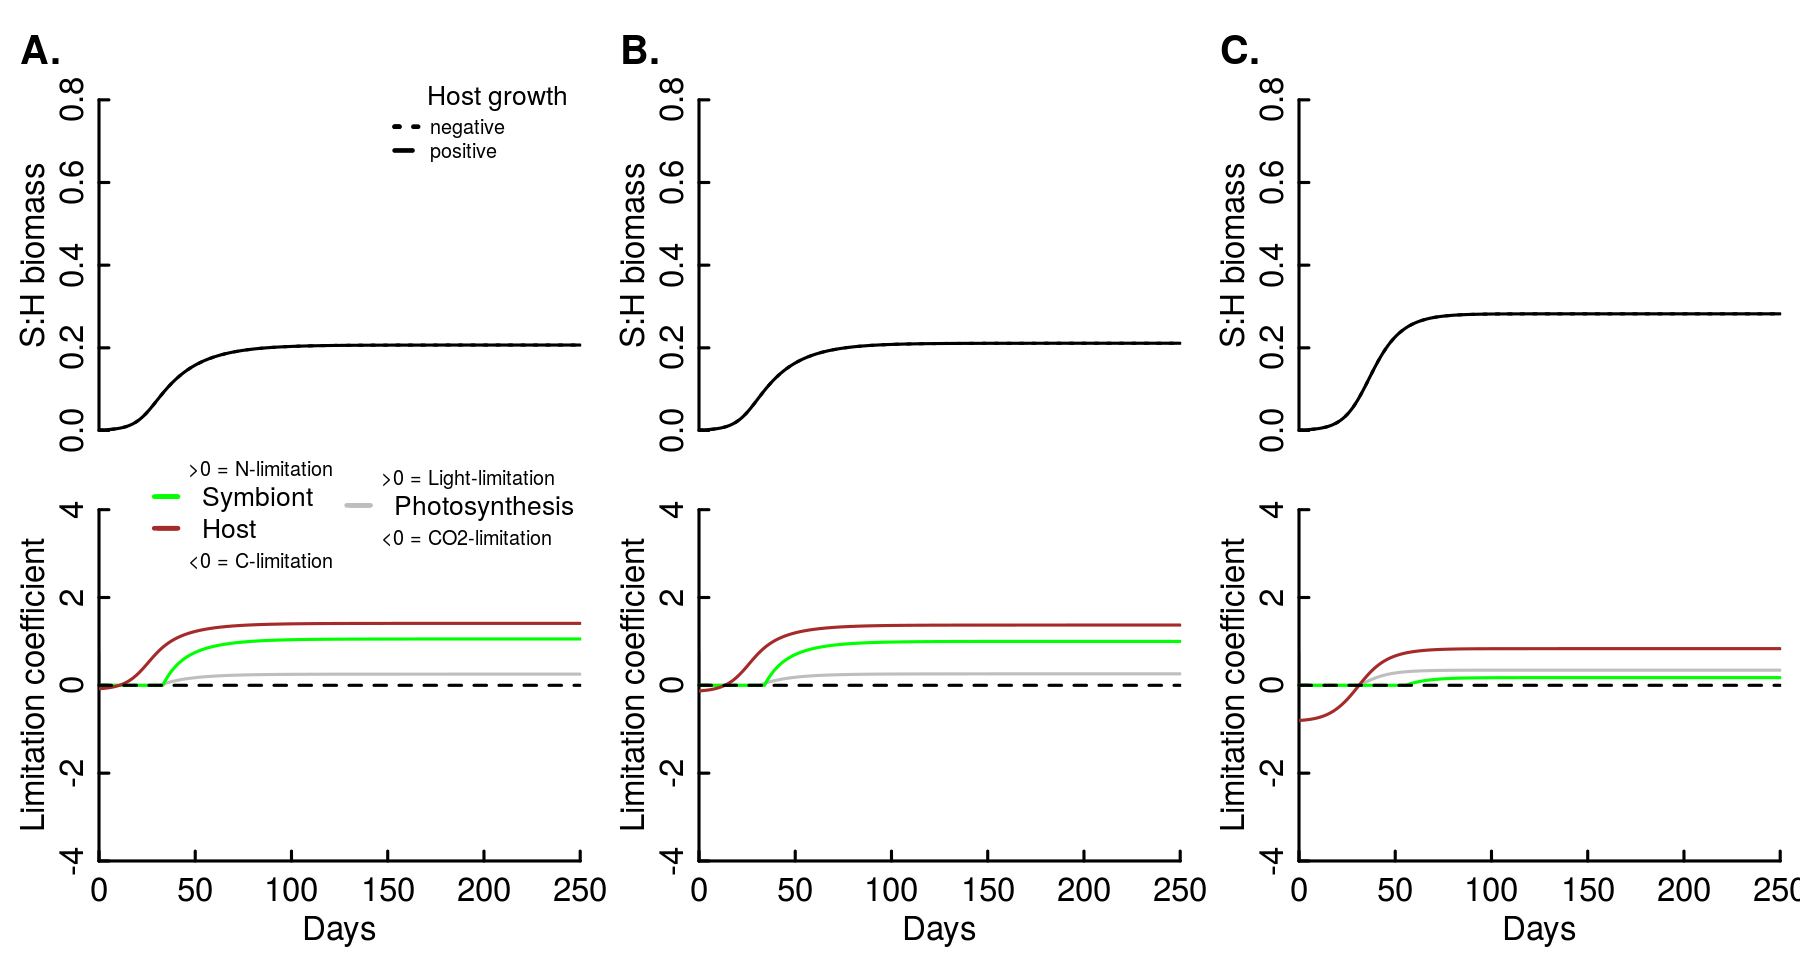
\includegraphics{../img/Fig8.png}
\caption{Hysteresis under different nutrient and feeding regimes. Steady
state S:H biomass ratios in constant environments with (A) low DIN (1e-7
M) and low food (2e-7 M), (B) low DIN (1e-7 M) and no food, (C) high DIN
(2e-6 M) and low food (2e-7 M), and (D) high DIN (2e-6 M) and high food
(4e-7 M). In each panel, steady states are shown starting from both high
initial S:H biomass (1, i.e.~healthy corals - closed circles) and low
initial initial S:H biomass (0.0001, i.e.~bleached corals - open
circles). Points are colored according to whether the host exhibits
positive (black) or negative (red) growth at steady state.}
\end{figure}

Dynamic simulations of recovery reveal another interesting behavior of
the system: under some conditions, an `overshoot' occurs in which S:H
biomass temporarily increases beyond the ratio maintained in the
`healthy' state, before returning to stabilize at this value (Fig. 9).
In fact, unusually high symbiont densities have been observed following
bleaching in both experimental (Cunning, Silverstein, and Baker 2015)
and field studies (Kemp et al. 2014), and have been interpreted as a
potential `disequilibrium in host-symbiont regulation' (Kemp et al.
2014). The model reveals the dynamics of this `overshoot' as follows: as
symbionts repopulate the host, photosynthesis becomes increasingly
CO\textsubscript{2}-limited due to weak CCM activity of the
carbon-limited host. Thus, although symbiont growth is not yet
carbon-limited, a growing symbiont population has less and less excess
carbon (per symbiont) to share, and is thus moving toward
carbon-limitation. Meanwhile, because S:H biomass is increasing, the
host receives more and more carbon per unit host biomass, and is thus
moving away from carbon-limitation. If the host overcomes
carbon-limitation \emph{before} the symbiont reaches it, then the system
rapidly transitions to the nitrogen-limited state and the S:H ratio
stabilizes without an overshoot (Fig. 9A). However, if the symbiont
becomes carbon-limited first (Fig. 9B, 9C), then carbon translocation
per symbiont declines further and photosynthesis becomes more
CO\textsubscript{2}-limited, which maintains carbon-limitation of the
host. In this situation, continued growth of less and less productive
symbionts drives S:H biomass to a much higher level before the host
finally overcomes carbon-limitation. At this point, representing the
peak of the overshoot, the transition to nitrogen-limitation finally
takes place and the S:H biomass ratio declines and stabilizes as
positive growth is resumed.

Whether this `overshoot' occurs or not is determined by the relative
availability of carbon and nitrogen to the host -- any factor that
enhances carbon-limitation of host growth (e.g.~high DIN and/or low
feeding) therefore magnifies the overshoot and prolongs the
dysfunctional, carbon-limited state of the symbiosis (Fig. 9). On the
other hand, factors that favor nitrogen-limitation, such as low external
DIN and/or high feeding rates, will accelerate the re-establishment of
nitrogen-limitation and prevent an overshoot from occurring at all.
While many scenarios are possible under different environmental
conditions, we illustrate the general effects of varying N and C
availability on recovery from bleaching with a series of simulations
that vary the N:C ratio of host's heterotrophic food source (Fig. 9A-C):
lower N:C ratios (effectively representing lower DIN and/or higher
heterotrophy) favor nitrogen-limitation and more rapid recovery, while
higher N:C ratios (effectively representing higher DIN and/or lower
heterotrophy) favor carbon-limitation and prolonged recovery with a
larger overshoot in S:H biomass.

\begin{figure}[htbp]
\centering
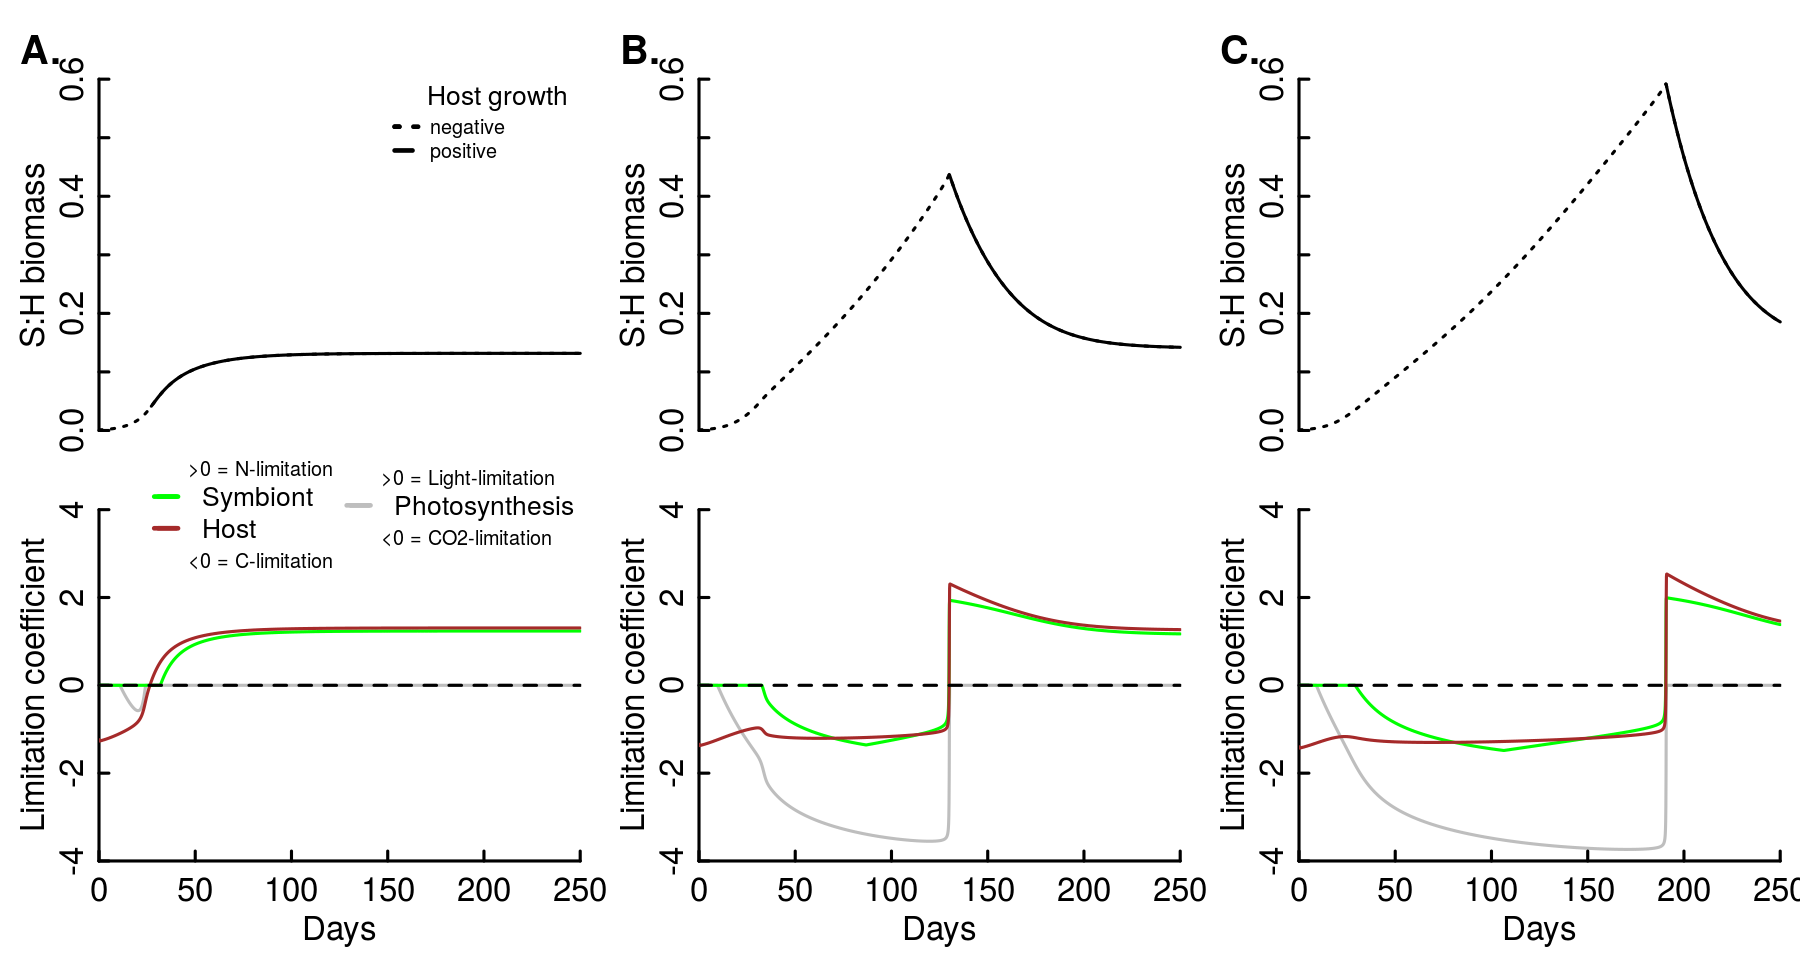
\includegraphics{../img/Fig9.png}
\caption{Recovery from bleaching with varying N:C availability (A:
N:C=0.100; B: N:C=0.175; C: N:C=0.220). Higher N:C ratios in a
heterotrophic food source (effectively representing higher external DIN
and/or lower feeding rates) cause a larger overshoot in the S:H biomass
ratio, and prolong the duration of time until the system `recovers' by
re-establishing nitrogen-limitation. Substrate limitation coefficients
were calculated using Eq. 23. All simulations were run with default
parameters (except varying \(n_{NX}\)), with L=20 mol photons
m\textsuperscript{2} d\textsuperscript{-1}, DIN=1e-7 mol N
L\textsuperscript{-1}, prey=1e-7 CmolX L\textsuperscript{-1}, and
initial S:H biomass=0.001.}
\end{figure}

These dynamics reveal that the re-establishment of nitrogen-limitation
is the most important diagnostic of recovery to a `healthy' state, as
this is when positive growth rates are resumed. A high S:H biomass ratio
alone does not necessarily indicate that a `healthy' state has been
reached, since the carbon-limited state may still persist (e.g.~Fig. 8B,
8C). This could explain why corals that have recovered their symbiont
populations after bleaching may still exhibit energetic deficits and
physiological impacts, possibly for months to years (Levitan et al.
2014, Hughes and Grottoli (2013))). These findings suggest that host
acquisition of carbon from a source other than the symbiont may be
extremely important for the system to recover from bleaching. Indeed,
host feeding has been shown to promote a more rapid return to
pre-bleaching levels of key physiological parameters in recovering
corals (Connolly, Lopez-Yglesias, and Anthony 2012). Additional carbon
sources for the host, such as direct uptake of dissolved organic carbon
(Levas et al. 2015), may also promote more rapid recovery from a
bleached state.

\section{Conclusions}\label{conclusions}

This dynamic bioenergetic model of coral-\emph{Symbiodinium} symbioses
mechanistically reproduces patterns in steady-state coral growth and
symbiont abundance commonly observed in corals, including higher
symbiont abundance with higher nutrients and feeding, lower symbiont
abundance with increasing light, and optimal growth at intermediate
light levels. Moreover, the model reproduces complex dynamic behaviors
including seasonal changes in symbiont density at different nutrient
levels, rapid bleaching above a threshold of high light, mitigation of
bleaching by heterotrophic feeding, exacerbation of bleaching by
elevated nutrients, and an overshoot of symbiont density during recovery
from bleaching. These examples demonstrate the model's ability to
integrate multiple environmental forcing functions to reproduce complex
responses; meanwhile, the diversity of these phenomena suggest the model
has captured many of the important features of the system in a unifying
mechanistic framework. This model also provides a new conceptual
framework for considering coral bleaching as a transition to an
alternate stable state, which has important implications for
understanding the performance and maintenance of symbiotic interactions.
In this context, the `healthy' stable state represents a scenario in
which nitrogen-limitation stabilizes the symbiont to host biomass ratio
and maintains positive growth. Conversely, carbon-limitation represents
a dysfunctional state wherein positive feedbacks result in coral
bleaching and negative growth, with hysteresis maintaining this
alternate state until a favorable environment is re-established.
Interestingly, alternate stable states have received much attention in
coral reef community ecology with respect to coral- and
macroalgal-dominance on reefs (Mumby, Hastings, and Edwards 2007). Here,
we find that the same principles may also mediate bleaching and recovery
in individual corals.

The model developed here can be used to explore many different dynamic
environmental scenarios, and represents a tool that biologists and
ecologists can use to generate hypotheses and make predictions in both
experimental and natural settings. Moreover, parameter values can be
modified to correspond to different genetic or functional types of coral
hosts and \emph{Symbiodinium} partners in order to evaluate variability
in system responses. Thus, the diversity of potential applications for
this model is high, and we envision this work as a foundation for
continued development, which may include more detailed treatments of
specific modules (e.g., DIC processing), and the incorporation of more
external forcing capabilities (e.g., external DIC, temperature).
Importantly, open source R code allows this effort to benefit from
contributions from the wider scientific community, including those with
empirical and theoretical backgrounds. Ultimately, the continued
refinement of these tools is fundamental in elucidating the mechanisms
of symbiosis function and dysfunction, and in predicting coral responses
to environmental change.

\section{Acknowledgements}\label{acknowledgements}

This work was supported by a NSF Postdoctoral Research Fellowship in
Biology to RC (\#1400787).

\section*{References}\label{references}
\addcontentsline{toc}{section}{References}

\hypertarget{refs}{}
\hypertarget{ref-Anthony:2002tc}{}
Anthony, K. 2002. ``Comparative analysis of energy allocation to tissue
and skeletal growth in corals.'' \emph{Limnology and Oceanography} 47
(5): 1417--29.
\url{https://www.scopus.com/inward/record.uri?partnerID=HzOxMe3b\&scp=0036733455\&origin=inward}.

\hypertarget{ref-ArmozaZvuloni:2014ju}{}
Armoza-Zvuloni, Rachel, Esti Kramarsky-Winter, Yossi Loya, Ami
Schlesinger, and Hanna Rosenfeld. 2014. ``Trioecy, a unique breeding
strategy in the sea anemone Aiptasia diaphana and its association with
sex steroids.'' \emph{Biology of Reproduction} 90 (6). Society for the
Study of Reproduction: 122--22.
doi:\href{https://doi.org/10.1095/biolreprod.113.114116}{10.1095/biolreprod.113.114116}.

\hypertarget{ref-Bak:1976bv}{}
Bak, R. 1976. ``The growth of coral colonies and the importance of
crustose coralline algae and burrowing sponges in relation with
carbonate accumulation.'' \emph{Netherlands Journal of Sea Research} 10
(3): 285--337.
doi:\href{https://doi.org/10.1016/0077-7579(76)90009-0}{10.1016/0077-7579(76)90009-0}.

\hypertarget{ref-Baker:2015kp}{}
Baker, Andrew C, and Ross Cunning. 2015. ``Coral 'Bleaching' as a
Generalized Stress Response to Environmental Disturbance.'' In
\emph{Diseases of Coral}, 396--409. Hoboken, NJ: John Wiley \& Sons,
Inc.
doi:\href{https://doi.org/10.1002/9781118828502.ch30}{10.1002/9781118828502.ch30}.

\hypertarget{ref-Baker:1975ip}{}
Baker, P, and Jon N Weber. 1975. ``Coral growth rate: Variation with
depth.'' \emph{Earth and Planetary Science Letters} 27 (1): 57--61.
doi:\href{https://doi.org/10.1016/0012-821X(75)90160-0}{10.1016/0012-821X(75)90160-0}.

\hypertarget{ref-Barott:2014gx}{}
Barott, Katie L, Alexander A Venn, Sidney O Perez, Sylvie Tambutte, and
Martin Tresguerres. 2014. ``Coral host cells acidify symbiotic algal
microenvironment to promote photosynthesis.'' \emph{Proceedings Of The
National Academy Of Sciences Of The United States Of America}, December.
National Acad Sciences, 201413483.
doi:\href{https://doi.org/10.1073/pnas.1413483112}{10.1073/pnas.1413483112}.

\hypertarget{ref-Borell:2008p108}{}
Borell, Esther M, Ade Yuliantri, Kai Bischof, and Claudio Richter. 2008.
``The effect of heterotrophy on photosynthesis and tissue composition of
two scleractinian corals under elevated temperature.'' \emph{Journal of
Experimental Marine Biology and Ecology} 364: 116--23.

\hypertarget{ref-Brown:1999p3534}{}
Brown, Barbara E, R P Dunne, I Ambarsari, Martin Le Tissier, and U
Satapoomin. 1999. ``Seasonal fluctuations in environmental factors and
variations in symbiotic algae and chlorophyll pigments in four
Indo-Pacific coral species.'' \emph{Marine Ecology Progress Series} 191:
53--69.

\hypertarget{ref-Butow:1998gz}{}
Butow, B, D Wynne, A Sukenik, O Hadas, and E Tel-Or. 1998. ``The
synergistic effect of carbon concentration and high temperature on lipid
peroxidation in Peridinium gatunense.'' \emph{Journal of Plankton
Research} 20 (2). Oxford University Press: 355--69.
doi:\href{https://doi.org/10.1093/plankt/20.2.355}{10.1093/plankt/20.2.355}.

\hypertarget{ref-Coles:1978p1124}{}
Coles, SL, and Paul L Jokiel. 1978. ``Synergistic effects of
temperature, salinity and light on the hermatypic coral Montipora
verrucosa.'' \emph{Marine Biology} 49: 187--95.
\url{http://www.springerlink.com/index/LU582837924G7674.pdf}.

\hypertarget{ref-Connolly:2012ep}{}
Connolly, Sean R, M A Lopez-Yglesias, and Kenneth R N Anthony. 2012.
``Food availability promotes rapid recovery from thermal stress in a
scleractinian coral.'' \emph{Coral Reefs} 31 (4). Springer-Verlag:
951--60.
doi:\href{https://doi.org/10.1007/s00338-012-0925-9}{10.1007/s00338-012-0925-9}.

\hypertarget{ref-Costanza:2014ex}{}
Costanza, R, R de Groot, and P Sutton. 2014. ``Changes in the global
value of ecosystem services.'' \emph{Global Environmental Change} 26:
152--58.
doi:\href{https://doi.org/10.1016/j.gloenvcha.2014.04.002}{10.1016/j.gloenvcha.2014.04.002}.

\hypertarget{ref-Cunning:2013gp}{}
Cunning, Ross, and Andrew C Baker. 2013. ``Excess algal symbionts
increase the susceptibility of reef corals to bleaching.'' \emph{Nature
Climate Change} 3 (March): 259--62.
doi:\href{https://doi.org/10.1038/nclimate1711}{10.1038/nclimate1711}.

\hypertarget{ref-Cunning:2015ja}{}
Cunning, Ross, Rachel N Silverstein, and Andrew C Baker. 2015.
``Investigating the causes and consequences of symbiont shuffling in a
multi-partner reef coral symbiosis under environmental change.''
\emph{Proceedings of the Royal Society B} 282: 20141725.
doi:\href{https://doi.org/10.1098/rspb.2014.1725\%7B/\&\%7Ddomain=pdf\%7B/\&\%7Ddate_stamp}{10.1098/rspb.2014.1725\{\textbackslash{}\&\}domain=pdf\{\textbackslash{}\&\}date\_stamp}.

\hypertarget{ref-Downs:2013kc}{}
Downs, C A, Kathleen E McDougall, Cheryl M Woodley, John E Fauth, Robert
H Richmond, Ariel Kushmaro, Stuart W Gibb, Yossi Loya, Gary K Ostrander,
and Esti Kramarsky-Winter. 2013. ``Heat-Stress and Light-Stress Induce
Different Cellular Pathologies in the Symbiotic Dinoflagellate during
Coral Bleaching.'' \emph{PLoS ONE} 8 (12): e77173.
doi:\href{https://doi.org/10.1371/journal.pone.0077173}{10.1371/journal.pone.0077173}.

\hypertarget{ref-Edmunds:2011bv}{}
Edmunds, Peter J, Hollie M Putnam, Roger M Nisbet, and Erik B Muller.
2011. ``Benchmarks in organism performance and their use in comparative
analyses.'' \emph{Oecologia} 167 (2): 379--90.
doi:\href{https://doi.org/10.1007/s00442-011-2004-2}{10.1007/s00442-011-2004-2}.

\hypertarget{ref-Enriquez:2005p142}{}
Enríquez, Susana, Eugenio R Méndez, and Roberto Iglesias-Prieto. 2005.
``Multiple scattering on coral skeletons enhances light absorption by
symbiotic algae.'' \emph{Limnology and Oceanography} 50 (4): 1025--32.

\hypertarget{ref-Eynaud:2011tv}{}
Eynaud, Yoan, Roger M Nisbet, and Erik B Muller. 2011. ``Impact of
excess and harmful radiation on energy budgets in scleractinian
corals.'' \emph{Ecological Modelling} 222 (7). Elsevier: 1315--22.
\url{http://www.sciencedirect.com/science/article/pii/S0304380011000263}.

\hypertarget{ref-Fagoonee:1999p4136}{}
Fagoonee, I, H B Wilson, M P Hassell, and J R Turner. 1999. ``The
Dynamics of Zooxanthellae Populations: A Long-Term Study in the Field.''
\emph{Science} 283 (5403): 843--45.
doi:\href{https://doi.org/10.1126/science.283.5403.843}{10.1126/science.283.5403.843}.

\hypertarget{ref-FerrierPages:2000p1950}{}
Ferrier-Pagès, Christine, Jean-Pierre Gattuso, S Dallot, and Jean
Jaubert. 2000. ``Effect of nutrient enrichment on growth and
photosynthesis of the zooxanthellate coral Stylophora \ldots{}.''
\emph{Coral Reefs}.
\url{http://www.springerlink.com/index/3DRC3K1Q57TPC0UT.pdf}.

\hypertarget{ref-Fitt:2001p832}{}
Fitt, William K, Barbara E Brown, Mark E Warner, and R P Dunne. 2001.
``Coral bleaching: interpretation of thermal tolerance limits and
thermal thresholds in tropical corals.'' \emph{Coral Reefs} 20: 51--65.

\hypertarget{ref-Fitt:2000p3792}{}
Fitt, William K, F K McFarland, Mark E Warner, and Geoff C Chilcoat.
2000. ``Seasonal patterns of tissue biomass and densities of symbiotic
dinoflagellates in reef corals and relation to coral bleaching.''
\emph{Limnology and Oceanography} 45 (3): 677--85.

\hypertarget{ref-Grottoli:2006p3692}{}
Grottoli, Andréa G, Lisa J Rodrigues, and James E Palardy. 2006.
``Heterotrophic plasticity and resilience in bleached corals.''
\emph{Nature} 440 (7088): 1186--9.
doi:\href{https://doi.org/10.1038/nature04565}{10.1038/nature04565}.

\hypertarget{ref-Hawkins:2016jj}{}
Hawkins, Thomas D, Julia C G Hagemeyer, Kenneth D Hoadley, Adam G Marsh,
and Mark E Warner. 2016. ``Partitioning of Respiration in an
Animal-Algal Symbiosis: Implications for Different Aerobic Capacity
between Symbiodinium spp.'' \emph{Frontiers in Physiology} 7 (April).
Frontiers: 125.
doi:\href{https://doi.org/10.3389/fphys.2016.00128}{10.3389/fphys.2016.00128}.

\hypertarget{ref-HoeghGuldberg:1999p4222}{}
Hoegh-Guldberg, Ove. 1999. ``Climate change, coral bleaching and the
future of the world's coral reefs.'' \emph{Marine and Freshwater
Research} 50 (November): 839--66.

\hypertarget{ref-Hopkinson:2015ev}{}
Hopkinson, Brian M, Anna L Tansik, and William K Fitt. 2015. ``Internal
carbonic anhydrase activity in the tissue of scleractinian corals is
sufficient to support proposed roles in photosynthesis and
calcification.'' \emph{The Journal of Experimental Biology}, April. The
Company of Biologists Ltd, jeb.118182.
doi:\href{https://doi.org/10.1242/jeb.118182}{10.1242/jeb.118182}.

\hypertarget{ref-Hughes:2013hd}{}
Hughes, Adam D, and Andréa G Grottoli. 2013. ``Heterotrophic
Compensation: A Possible Mechanism for Resilience of Coral Reefs to
Global Warming or a Sign of Prolonged Stress?'' \emph{PLoS ONE} 8 (11).
Public Library of Science: e81172.
doi:\href{https://doi.org/10.1371/journal.pone.0081172}{10.1371/journal.pone.0081172}.

\hypertarget{ref-Huston:1985ec}{}
Huston, M. 1985. ``Variation in coral growth rates with depth at
Discovery Bay, Jamaica.'' \emph{Coral Reefs} 4 (1): 19--25.
doi:\href{https://doi.org/10.1007/BF00302200}{10.1007/BF00302200}.

\hypertarget{ref-Jager:2013bj}{}
Jager, Tjalling, Benjamin T Martin, and Elke I Zimmer. 2013. ``DEBkiss
or the quest for the simplest generic model of animal life history.''
\emph{Journal of Theoretical Biology} 328: 9--18.
doi:\href{https://doi.org/10.1016/j.jtbi.2013.03.011}{10.1016/j.jtbi.2013.03.011}.

\hypertarget{ref-Jokiel:1977p7353}{}
Jokiel, Paul L, and SL Coles. 1977. ``Effects of temperature on the
mortality and growth of Hawaiian reef corals.'' \emph{Marine Biology} 43
(3): 201--8.

\hypertarget{ref-Jones:1998p3572}{}
Jones, Ross J, Ove Hoegh-Guldberg, Anthony W D Larkum, and Ulrich
Schreiber. 1998. ``Temperature-induced bleaching of corals begins with
impairment of the CO2 fixation mechanism in zooxanthellae.''
\emph{Plant, Cell and Environment} 21 (12): 1219--30.

\hypertarget{ref-Kemp:2014ug}{}
Kemp, Dustin W, X Hernandez-Pech, Roberto Iglesias-Prieto, William K
Fitt, and Gregory W Schmidt. 2014. ``Community dynamics and physiology
of Symbiodinium spp. before, during, and after a coral bleaching
event.'' \emph{Limnology and Oceanography}.
\url{http://www.aslo.org/lo/pdf/vol_59/issue_3/0788.pdf}.

\hypertarget{ref-Kooijman:2010vd}{}
Kooijman, SALM. 2010. \emph{Dynamic Energy Budget Theory for Metabolic
Organization}. 3rd ed. Cambridge University Press.

\hypertarget{ref-Lesser:1997p3587}{}
Lesser, Michael P. 1997. ``Oxidative stress causes coral bleaching
during exposure to elevated temperatures.'' \emph{Coral Reefs} 16
(July): 187--92.

\hypertarget{ref-Levas:2015ic}{}
Levas, Stephen, Andréa G Grottoli, Verena Schoepf, Matthew D
Aschaffenburg, Justin Baumann, James E Bauer, and Mark E Warner. 2015.
``Can heterotrophic uptake of dissolved organic carbon and zooplankton
mitigate carbon budget deficits in annually bleached corals?''
\emph{Coral Reefs} 35 (2). Springer Berlin Heidelberg: 495--506.
doi:\href{https://doi.org/10.1007/s00338-015-1390-z}{10.1007/s00338-015-1390-z}.

\hypertarget{ref-Levitan:2014et}{}
Levitan, D R, W Boudreau, J Jara, and Nancy Knowlton. 2014. ``Long-term
reduced spawning in Orbicella coral species due to temperature stress.''
\emph{Marine Ecology Progress Series} 515: 1--10.
doi:\href{https://doi.org/10.3354/meps11063}{10.3354/meps11063}.

\hypertarget{ref-Marcelino:2013hz}{}
Marcelino, Luisa A, Mark W Westneat, Valentina Stoyneva, Jillian Henss,
Jeremy D Rogers, Andrew Radosevich, Vladimir Turzhitsky, et al. 2013.
``Modulation of Light-Enhancement to Symbiotic Algae by Light-Scattering
in Corals and Evolutionary Trends in Bleaching.'' \emph{PLoS ONE} 8 (4):
e61492.
doi:\href{https://doi.org/10.1371/journal.pone.0061492.s008}{10.1371/journal.pone.0061492.s008}.

\hypertarget{ref-Marubini:1996p8460}{}
Marubini, F, and PS Davies. 1996. ``Nitrate increases zooxanthellae
population density and reduces skeletogenesis in corals.'' \emph{Marine
Biology} 127 (2): 319--28.
\url{http://www.scopus.com/inward/record.url?partnerID=yv4JPVwI\&eid=2-s2.0-0030301761\&md5=0971551a6865f30046294b9e17fb4081}.

\hypertarget{ref-Muller:2009io}{}
Muller, Erik B, Sebastiaan A L M Kooijman, Peter J Edmunds, Francis J
Doyle, and Roger M Nisbet. 2009. ``Dynamic energy budgets in syntrophic
symbiotic relationships between heterotrophic hosts and photoautotrophic
symbionts.'' \emph{Journal of Theoretical Biology} 259 (1): 44--57.
doi:\href{https://doi.org/10.1016/j.jtbi.2009.03.004}{10.1016/j.jtbi.2009.03.004}.

\hypertarget{ref-MullerParker:1987cr}{}
Muller-Parker, Gisèle. 1987. ``Seasonal variation in light-shade
adaptation of natural populations of the symbiotic sea anemone
Aiptasiapulchella (Carlgren, 1943) in Hawaii.'' \emph{Journal of
Experimental Marine Biology and Ecology} 112 (2): 165--83.
doi:\href{https://doi.org/10.1016/0022-0981(87)90115-8}{10.1016/0022-0981(87)90115-8}.

\hypertarget{ref-MullerParker:1994uo}{}
Muller-Parker, Gisèle, Lawrence R McCloskey, Ove Hoegh-Guldberg, and PJ
McAuley. 1994. ``Effect of ammonium enrichment on animal and algal
biomass of the coral Pocillopora damicornis.'' \emph{Pacific Science} 48
(3). \url{http://scholarspace.manoa.hawaii.edu/handle/10125/2236}.

\hypertarget{ref-Mumby:2007cr}{}
Mumby, Peter J, Alan Hastings, and Helen J. Edwards. 2007. ``Thresholds
and the resilience of Caribbean coral reefs.'' \emph{Nature} 450 (7166).
Nature Publishing Group: 98--101.
doi:\href{https://doi.org/10.1038/nature06252}{10.1038/nature06252}.

\hypertarget{ref-Muscatine:1977p4220}{}
Muscatine, Leonard, and James W Porter. 1977. ``Reef corals: mutualistic
symbioses adapted to nutrient-poor environments.'' \emph{Bioscience} 27
(7): 454--60.

\hypertarget{ref-Muscatine:1981jy}{}
Muscatine, Leonard, L R McCloskey, and R E Marian. 1981. ``Estimating
the daily contribution of carbon from zooxanthellae to coral animal
respiration.'' \emph{Limnology and Oceanography} 26 (4): 601--11.
doi:\href{https://doi.org/10.4319/lo.1981.26.4.0601}{10.4319/lo.1981.26.4.0601}.

\hypertarget{ref-Osinga:2011kq}{}
Osinga, Ronald, Miriam Schutter, Ben Griffioen, René H Wijffels, Johan A
J Verreth, Shai Shafir, Stéphane Henard, Maura Taruffi, Claudia Gili,
and Silvia Lavorano. 2011. ``The Biology and Economics of Coral
Growth.'' \emph{Marine Biotechnology} 13 (4): 658--71.
doi:\href{https://doi.org/10.1007/s10126-011-9382-7}{10.1007/s10126-011-9382-7}.

\hypertarget{ref-Osinga:2012is}{}
Osinga, Ronald, Miriam Schutter, Tim Wijgerde, Buki Rinkevich, Shai
Shafir, Muki Shpigel, Gian Marco Luna, et al. 2012. ``The CORALZOO
project: a synopsis of four years of public aquarium science.''
\emph{Journal of the Marine Biological Association of the UK} 92 (04).
Cambridge University Press: 753--68.
doi:\href{https://doi.org/10.1017/S0025315411001779}{10.1017/S0025315411001779}.

\hypertarget{ref-Powles:1984tm}{}
Powles, Stephen B. 1984. ``Photoinhibition of photosynthesis induced by
visible light.'' \emph{Annual Review of Plant Physiology} 35: 15--44.

\hypertarget{ref-RALanguageandEn:2014wf}{}
R Core Team. 2014. ``R: A Language and Environment for Statistical
Computing.'' Vienna, Austria: R Foundation for Statistical Computing.
\url{http://www.R-project.org/}.

\hypertarget{ref-Roth:2014wf}{}
Roth, M S. 2014. ``The engine of the reef: Photobiology of the
coral-algal symbiosis.'' \emph{Frontiers in Microbiology}.
\url{http://journal.frontiersin.org/Journal/10.3389/fmicb.2014.00422/pdf}.

\hypertarget{ref-Schutter:2010p7758}{}
Schutter, M, J Crocker, A Paijmans, M Janse, R Osinga, A J Verreth, and
R H Wijffels. 2010. ``The effect of different flow regimes on the growth
and metabolic rates of the scleractinian coral Galaxea fascicularis.''
\emph{Coral Reefs}, April.
doi:\href{https://doi.org/10.1007/s00338-010-0617-2}{10.1007/s00338-010-0617-2}.

\hypertarget{ref-Schutter:2011ie}{}
Schutter, Miriam, Rosa M van der Ven, Max Janse, Johan A J Verreth, René
H Wijffels, and Ronald Osinga. 2011. ``Light intensity, photoperiod
duration, daily light flux and coral growth of Galaxea fascicularis in
an aquarium setting: a matter of photons?'' \emph{Journal of the Marine
Biological Association of the UK} 92 (04). Cambridge University Press:
703--12.
doi:\href{https://doi.org/10.1017/S0025315411000920}{10.1017/S0025315411000920}.

\hypertarget{ref-Shantz:2015dz}{}
Shantz, Andrew A, Nathan P Lemoine, and Deron E Burkepile. 2015.
``Nutrient loading alters the performance of key nutrient exchange
mutualisms.'' \emph{Ecology Letters} 19 (1): 20--28.
doi:\href{https://doi.org/10.1111/ele.12538}{10.1111/ele.12538}.

\hypertarget{ref-Stimson:1997p3837}{}
Stimson, J. 1997. ``The annual cycle of density of zooxanthellae in the
tissues of field and laboratory-held Pocillopora damicornis
(Linnaeus).'' \emph{Journal of Experimental Marine Biology and Ecology}
214 (1-2): 35--48.

\hypertarget{ref-Tanaka:2013dj}{}
Tanaka, Yasuaki, Akira Iguchi, Mayuri Inoue, Chiharu Mori, K Sakai,
Atsushi Suzuki, Hodaka Kawahata, and Takashi Nakamura. 2013. ``Marine
Pollution Bulletin.'' \emph{Marine Pollution Bulletin} 68 (1-2): 93--98.
doi:\href{https://doi.org/10.1016/j.marpolbul.2012.12.017}{10.1016/j.marpolbul.2012.12.017}.

\hypertarget{ref-Tanaka:2007uv}{}
Tanaka, Yasuaki, Toshihiro Miyajima, Isao Koike, Takeshi Hayashibara,
and Hiroshi Ogawa. 2007. ``Imbalanced coral growth between organic
tissue and carbonate skeleton caused by nutrient enrichment.''
\emph{Limnology and Oceanography}.
\url{http://www.aslo.org/lo/toc/vol_52/issue_3/1139.pdf}.

\hypertarget{ref-Tansik:2015cm}{}
Tansik, Anna L, William K Fitt, and Brian M Hopkinson. 2015. ``External
carbonic anhydrase in three Caribbean corals: quantification of activity
and role in CO2 uptake.'' \emph{Coral Reefs} 34 (3). Springer Berlin
Heidelberg: 703--13.
doi:\href{https://doi.org/10.1007/s00338-015-1289-8}{10.1007/s00338-015-1289-8}.

\hypertarget{ref-Titlyanov:2001p3631}{}
Titlyanov, E A, T V Titlyanova, K Yamazato, and Robert van Woesik. 2001.
``Photo-acclimation dynamics of the coral Stylophora pistillata to low
and extremely low light.'' \emph{Journal of Experimental Marine Biology
and Ecology} 263 (2): 211--25.

\hypertarget{ref-VegaThurber:2014hk}{}
Vega Thurber, Rebecca L, Deron E Burkepile, Corinne Fuchs, Andrew A
Shantz, Ryan McMinds, and Jesse R Zaneveld. 2014. ``Chronic nutrient
enrichment increases prevalence and severity of coral disease and
bleaching.'' \emph{Global Change Biology} 20 (2): 544--54.
doi:\href{https://doi.org/10.1111/gcb.12450}{10.1111/gcb.12450}.

\hypertarget{ref-Wang:1998p128}{}
Wang, J, and Angela E Douglas. 1998. ``Nitrogen recycling or nitrogen
conservation in an alga-invertebrate symbiosis?'' \emph{The Journal of
Experimental Biology} 201: 2445--53.

\hypertarget{ref-Warner:1999p4239}{}
Warner, Mark E, William K Fitt, and Gregory W Schmidt. 1999. ``Damage to
photosystem II in symbiotic dinoflagellates: A determinant of coral
bleaching.'' \emph{Proceedings Of The National Academy Of Sciences Of
The United States Of America} 96 (14): 8007--12.

\hypertarget{ref-Weis:2008p944}{}
Weis, Virginia M. 2008. ``Cellular mechanisms of Cnidarian bleaching:
stress causes the collapse of symbiosis.'' \emph{The Journal of
Experimental Biology} 211 (Pt 19): 3059--66.
doi:\href{https://doi.org/10.1242/jeb.009597}{10.1242/jeb.009597}.

\hypertarget{ref-Wiedenmann:2013bn}{}
Wiedenmann, Jörg, C D'Angelo, Edward G Smith, Alan N Hunt, François-Eric
Legiret, Anthony D Postle, and Eric P Achterberg. 2013. ``Nutrient
enrichment can increase the susceptibility of reef corals to
bleaching.'' \emph{Nature Climate Change} 3. Nature Publishing Group:
160--64.
doi:\href{https://doi.org/10.1038/nclimate1661}{10.1038/nclimate1661}.

\hypertarget{ref-Wooldridge:2009p7807}{}
Wooldridge, Scott A. 2009. ``A new conceptual model for the warm-water
breakdown of the coral-algae endosymbiosis.'' \emph{Marine and
Freshwater Research} 60 (June): 483--96.

\hypertarget{ref-Wooldridge:2010p7809}{}
---------. 2010. ``Is the coral-algae symbiosis really 'mutually
beneficial' for the partners?'' \emph{BioEssays}, May.

\hypertarget{ref-Wooldridge:2013tj}{}
---------. 2013. ``Breakdown of the coral-algae symbiosis: towards
formalising a linkage between warm-water bleaching thresholds and the
growth rate of the intracellular zooxanthellae.'' \emph{Biogeosciences}
10: 1647--58.
\url{http://www.biogeosciences.net/10/1647/2013/bg-10-1647-2013.html}.

\hypertarget{ref-Wooldridge:2014di}{}
---------. 2014a. ``Differential thermal bleaching susceptibilities
amongst coral taxa: re-posing the role of the host.'' \emph{Coral Reefs}
33 (1). Springer Berlin Heidelberg: 15--27.
doi:\href{https://doi.org/10.1007/s00338-013-1111-4}{10.1007/s00338-013-1111-4}.

\hypertarget{ref-Wooldridge:2014hc}{}
---------. 2014b. ``Formalising a mechanistic linkage between
heterotrophic feeding and thermal bleaching resistance.'' \emph{Coral
Reefs}. Springer Berlin Heidelberg, 1--6.
doi:\href{https://doi.org/10.1007/s00338-014-1193-7}{10.1007/s00338-014-1193-7}.

\hypertarget{ref-Wooldridge:2009kb}{}
Wooldridge, Scott A, and Terry J Done. 2009. ``Improved water quality
can ameliorate effects of climate change on corals.'' \emph{Ecological
Applications} 19 (6). Ecological Society of America: 1492--9.
doi:\href{https://doi.org/10.1890/08-0963.1}{10.1890/08-0963.1}.

\hypertarget{ref-Yellowlees:2008p331}{}
Yellowlees, David, T A V Rees, and William Leggat. 2008. ``Metabolic
interactions between algal symbionts and invertebrate hosts.''
\emph{Plant, Cell and Environment} 31: 679--94.

\end{document}


